\documentclass{article}
\usepackage[utf8]{inputenc}
\usepackage[absolute]{textpos}
\usepackage[default]{raleway}
\usepackage{titlesec, multirow, comment, tabularx, longtable, makecell, listings, array, setspace, geometry, graphicx, xcolor, xparse, fancyvrb, relsize, fancyhdr, booktabs, hyperref, float}
\usepackage{colortbl}
\usepackage{lipsum}
%\geometry{a4paper, left=2cm, right=2cm, top=2cm, bottom=2.5cm}
\renewcommand{\headrulewidth}{0pt}

% Definisci uno stile per i comandi git
\definecolor{light-gray}{gray}{0.92}

\lstdefinestyle{code}{
    frame=single,
    framesep=1mm,
    rulecolor=\color{light-gray},
    backgroundcolor=\color{light-gray},
    basicstyle=\ttfamily,
}

% ----------------------------- Definizione tabella ---------------------------

\newcolumntype{C}[1]{>{\centering\arraybackslash}m{#1}}
\newcolumntype{L}[1]{>{\raggedright\arraybackslash}m{#1}}

%\setcellgapes{2ex} % Imposta l'altezza dell'header (2ex)


% ------------------------------Metadati indice --------------------------------
\title{\textbf{\fontsize{28}{6}\selectfont Indice}}
\author{\fontsize{14}{6}\selectfont ByteOps}
\date{}


% -----------------------------Creazione footer --------------------------------

\pagestyle{fancy}
\fancyhf{}
\renewcommand{\footrulewidth}{0.4pt}
\lfoot{
    \parbox[c]{2cm}{
\includegraphics[width=2cm]{../Images/logo.png}}
    \textcolor[RGB]{120, 120, 120}{$\cdot$ Analisi dei requisiti}
}
\rfoot{\thepage}

% --------------------------Modifica formato hyperlinks ------------------------

\hypersetup{
    colorlinks=true,
    linkcolor=black,
    filecolor=black,      
    pdftitle={Analisi dei Requisiti},
    pdfpagemode=FullScreen,
}

% ------------------------------- Valore sotto-paragrafi indice --------------------------------------

\setcounter{secnumdepth}{4}
\setcounter{tocdepth}{4}

\titleformat{\section}
{\normalfont\huge\bfseries}{\thesection}{0.2cm}{}
\titlespacing*{\paragraph}{0pt}{0.5cm}{0.1cm}

\titleformat{\subsection}
{\normalfont\Large\bfseries}{\thesubsection}{0.2cm}{}
\titlespacing*{\paragraph}{0pt}{0.5cm}{0.1cm}

\titleformat{\subsubsection}
{\normalfont\large\bfseries}{\thesubsubsection}{0.2cm}{}
\titlespacing*{\paragraph}{0pt}{0.5cm}{0.1cm}

\titleformat{\paragraph}
{\normalfont\normalsize\bfseries}{\theparagraph}{0.2cm}{}
\titlespacing*{\paragraph}{0pt}{0.5cm}{0.1cm}

% ------------------------------- Front Page ---------------------------------------

\begin{document}

% --------------------------Aggiunta firma finale ------------------------
%\begin{textblock*}{\textwidth}(0.85\textwidth, 1.16\textheight)
%   Il responsabile: Nome Cognome
%\end{textblock*}
% ------------------------------------------------------------------------

\pagestyle{fancy}
\begin{center}
    
\includegraphics[width = 0.7\textwidth]{../Images/logo.png} \\
    \vspace{0.2cm}
    \textcolor[RGB]{60, 60, 60}{\textit{ByteOps.swe@gmail.com}} \\
    \vspace{1cm}
    \fontsize{16}{6}\selectfont Analisi dei requisiti\\
    \vspace{0.5cm}
\end{center}

\section*{Informazioni documento}
\def\arraystretch{1.2}
\begin{tabular}{>{\raggedleft\arraybackslash}p{0.2\textwidth}|>{\raggedright\arraybackslash}p{0.6\textwidth}c}
    \hline
    \addlinespace
    \textbf{Redattori}    & A. Barutta\\ & R.Smanio\\ & E.Hysa\\ & L. Skenderi\\ & F.Pozza \vspace{10pt} \\
    \textbf{Verificatori} & E. Hysa\\ & A.Barutta\\ & N.Preto\\ & D.Diotto\\ & L.Skenderi \vspace{10pt} \\
    \textbf{Destinatari}  & ByteOps\\ & T. Vardanega   \\ & R. Cardin \vspace{10pt} \\
\end{tabular}
\pagebreak

% ------------------------- Changelog ----------------------------

\section*{Registro delle modifiche}

\begin{longtable}{|C{1.5cm}|C{2.1cm}|C{2cm}|C{2cm}|C{5cm}|}
    \hline
    \textbf{Versione} & \textbf{Data} & \textbf{Autore} & \textbf{Verificatore} & \textbf{Dettaglio} \\
    \hline \hline
    \label{Git_Action_Version}1.0.0 
            & 12/01/2024    & \makecell{N, Preto}       & F. Pozza     & Revisione completa documento per RTB \\
    \hline            
    0.8.2   & 08/01/2024    & \makecell{F. Pozza}       & D. Diotto     & Correzioni grammaticali, impaginazione finale \\
    \hline            
    0.8.1   & 27/12/2023    & \makecell{F. Pozza}       & L. Skenderi   & Modfiche casi d'uso \\
    \hline
    0.8.0   & 18/12/2023    & \makecell{L. Skenderi}    & N. Preto      & Aggiunta Req. prestazionali \\
    \hline
    0.7.4   & 14/12/2023    & \makecell{L. Skenderi}    & A. Barutta    & Aggiustamenti Req. vincolo \\
    \hline
    0.7.3   & 14/12/2023    & \makecell{L. Skenderi}    & A. Barutta    & Aggiustamenti Req. qualità \\
    \hline
    0.7.2   & 12/12/2023    & \makecell{L. Skenderi}    & A. Barutta    & Aggiustamenti Req. Funzionali \\
    \hline
    0.7.1   & 10/12/2023    & \makecell{L. Skenderi}    & A. Barutta    & Aggiustamenti casi d'uso \\
    \hline
    0.7.0   & 09/12/2023    & \makecell{R. Smanio}      & D. Diotto & Riepilogo \\
    \hline
    0.6.0   & 08/12/2023    & \makecell{E. Hysa\\ R. Smanio}        & D. Diotto & Tracciamento \\
    \hline
    0.5.0   & 07/12/2023    & \makecell{E. Hysa\\ R. Smanio}        & D. Diotto & \makecell{Refactor sez. Req} \\
    \hline
    0.4.3   & 06/12/2023    & \makecell{E. Hysa\\ R. Smanio}        & D. Diotto & \makecell{Casi d'uso UC21, UC22, \\ UC23, UC24, UC25, UC26, \\ UC27, UC28, UC29} \\
    \hline
    0.4.3   & 05/12/2023    & \makecell{E. Hysa\\ R. Smanio}        & D. Diotto & \makecell{Casi d'uso UC18, UC19, \\ UC20 e sottocasi} \\
    \hline
    0.4.2   & 04/12/2023    & \makecell{E. Hysa\\ R. Smanio}        & D. Diotto & \makecell{Casi d'uso UC12, UC13 \\ e sottocasi} \\
    \hline
    0.4.1   & 02/12/2023    & \makecell{E. Hysa\\ R. Smanio}        & D. Diotto & \makecell{Refactor sottocasi di UC1} \\
    \hline
    0.4.0   & 01/12/2023    & \makecell{E. Hysa\\ R. Smanio}        & D. Diotto & \makecell{Refactor UC1, UC2} \\
    \hline
    0.3.0   & 25/11/2023    & \makecell{E. Hysa}                    & D. Diotto & \makecell{Sez. R. Vincolo} \\
    \hline
    0.2.0   & 22/11/2023    & \makecell{A. Barutta\\ R. Smanio}     & E. Hysa   & \makecell{Sez. R. Funzionali} \\
    \hline
    0.1.9   & 21/11/2023    & \makecell{A. Barutta\\ R. Smanio}     & E. Hysa   &  \makecell{Sottocasi di UC6, UC7} \\
    \hline
    0.1.8   & 21/11/2023    & \makecell{A. Barutta\\ R. Smanio}     & E. Hysa   &  \makecell{Casi d'uso UC6, UC7, \\ UC9, UC10} \\
    \hline
    0.1.7   & 20/11/2023    & \makecell{A. Barutta\\ R. Smanio}     & E. Hysa   &  \makecell{Sottocasi di UC1, UC2, UC3} \\
    \hline
    0.1.6   & 18/11/2023    & \makecell{A. Barutta\\ R. Smanio}     & E. Hysa   &  \makecell{Casi d'uso UC1, UC2, UC3} \\
    \hline
    0.1.5   & 17/11/2023    & \makecell{A. Barutta\\ R. Smanio}     & E. Hysa   &  \makecell{Obiettivi del prodotto} \\
    \hline
    0.1.4   & 16/11/2023    & \makecell{A. Barutta\\ R. Smanio}     & N. Preto  &  \makecell{Aggiunto glossario} \\
    \hline
    0.1.3   & 15/11/2023    & \makecell{A. Barutta\\ R. Smanio}     & N. Preto  &  \makecell{Integrazione di casi d'uso} \\
    \hline
    0.1.2   & 13/11/2023    & \makecell{A. Barutta\\ R. Smanio}     & N. Preto  &  \makecell{Casi d'uso} \\
    \hline
    0.1.1   & 12/11/2023    & \makecell{A. Barutta\\ R. Smanio}     & N. Preto  &  \makecell{Descrizione del Prodotto} \\
    \hline
    0.1.0   & 12/11/2023    & \makecell{A. Barutta\\ R. Smanio}     & N. Preto  &  \makecell{Introduzione} \\
    \hline
\end{longtable}
\pagebreak

% ------------------------- Generazione automatica indice ----------------------
\setstretch{1.5}
\maketitle
\thispagestyle{fancy}
\tableofcontents
\listoffigures % Indice delle figure
\setstretch{1.2}
\pagebreak

% ------------------------ INIZIO DOCUMENTO -----------------------
\flushleft

\section{Introduzione}

\subsection{Scopo del Manuale}
Il manuale ha lo scopo di assistere l’utente passo dopo passo per un corretto utilizzo del
software così da sfruttarne appieno tutte le funzionalità presenti per offrire un’esperienza
ottimale

\subsection{Glossario}
Incluso nella documentazione è presente il \textbf{\textit{Glossario}} in cui sono definiti tutti i termini specifici o eventualmente ambigui presenti nei vari documenti del progetto. Se un termine è nel \textbf{\textit{Glossario}}, viene segnalato con una \textit{G} a pedice accanto ad esso.

\subsubsection{Raccolta termini del glossario}
Il \textbf{\textit{Glossario}} verrà compilato attraverso un documento condiviso su \LaTeX \textsubscript{\textit{G}}, accessibile a ttti i membri del gruppo. Qui, verranno elencati i ter min  i di particolare rilevanza nel contesto del progetto, seguendo una checklist.   Successivamente, l'\textit{Amministratore} del progetto si occuperà di dettagliare  ulteriormente questi termini nella creazione del \textbf{\textit{Glossario}} ufficiale. 
\subsection{Riferimenti}
\subsubsection{Riferimenti informativi}
    \begin{itemize}
        \item \href {https://www.math.unipd.it/~tullio/IS-1/2023/Progetto/C6.pdf} {Capitolato d'appalto C6 - InnovaCity }
        \item \href{https://www.math.unipd.it/~tullio/IS-1/2023/Dispense/T4.pdf} {Slide del corso di Ingegneria del Software - Gestione di progetto }
        \item \href{https://www.math.unipd.it/~tullio/IS-1/2023/Dispense/T2.pdf} {Slide del corso di Ingegneria del Software - Ciclo di vita del software }
    \end{itemize}
 
\subsubsection{Riferimenti normativi}
    \begin{itemize}
    \item Norme di progetto
    \item \href {https://www.math.unipd.it/~tullio/IS-1/2023/Dispense/PD2.pdf} {Regolamento del progetto didattico }
    \end{itemize}

\vspace{0.5cm}


\section{Descrizione del prodotto}

\subsection{Obiettivi del prodotto}
Sviluppare una piattaforma di monitoraggio di una "Smart City" che consenta di avere sotto
controllo lo stato di salute della città in modo tale da prendere decisioni veloci, efficaci
ed analizzare poi gli effetti conseguenti.
A tale scopo il proponente richiede di simulare dei sensori posti in diverse aree per reperire
informazioni relative alle condizioni della città come, ad esempio, temperatura, umidità,
polveri sottili nell’aria, traffico, livelli di acqua, stato di riempimento delle isole ecologiche,
guasti elettrici e molto altro.
I dati trasmessi in tempo reale dai sensori devono poter essere memorizzati in un database
in modo tale da renderli disponibili per la visualizzazione tramite una dashboard, composta anche da widget e grafici, per una visione d’insieme delle condizioni della città in
tempo reale.
L’applicativo potrà consentire alle autorità locali di prendere decisioni informate e tempestive sulla gestione delle risorse e sull’implementazione di servizi e, inoltre, si potrebbe
rivelare uno strumento essenziale per coinvolgere i cittadini nella gestione e nel miglioramento della città.
\vspace{0.3cm}

L’implementazione di una città monitorata da sensori rappresenta un approccio promettente
nell’ottica di ottimizzare l’efficienza e la qualità della vita urbana. Tale sistema può consentire
una raccolta continua di dati e informazioni cruciali, fornendo una base solida per
l’ottimizzazione dei servizi pubblici, la gestione del traffico, la sicurezza e la sostenibilità
ambientale.



\input{Sottosezioni/Analisi_dei_requisiti/Funzionalità_del_prodotto.tex}

\subsection{Caratteristiche utente}
\textbf{Autorità Locali:} Gli utenti principali sono le autorità locali responsabili della gestione e del monitoraggio della Smart City. Questi utenti devono essere in grado di prendere decisioni informate sulla base delle informazioni raccolte e analizzate dal sistema.
\begin{itemize}
    \item L'utente dovrà utilizzare un dispositivo (Desktop o Mobile) connesso alla rete per poter accedere alla piattaforma.
\end{itemize}


\section{Tecnologie}
In questa sezione sono definiti gli strumenti e le tecnologie impiegati per lo sviluppo e l'implementazione del software relativo al progetto InnovaCity.

Si procederà quindi con la descrizione delle tecnologie e dei linguaggi di programmazione utilizzati, delle librerie e dei framework necessari, nonché delle infrastrutture richieste.

L'obiettivo principale è garantire che il software sia sviluppato utilizzando le tecnologie più appropriate e selezionando le opzioni ottimali in termini di efficienza, sicurezza e affidabilità.

\subsection{Docker}
Per lo sviluppo, il testing e il rilascio del prodotto sono stati utilizzati container Docker in modo tale da garantire ambienti consistenti e riproducibili.

\subsubsection{Ambienti}
\begin{itemize}
  \item \textbf{Ambiente di sviluppo:}
    \begin{itemize}
      \item È l'ambiente dove i software developer scrivono, testano e modificano il codice sorgente;
      \item Può includere strumenti di debug e monitoraggio per facilitare lo sviluppo e la correzione di errori;
      \item Non è accessibile agli utenti finali.
    \end{itemize}
    \item \textbf{Ambiente di test:}
    \begin{itemize}
      \item Simula l'ambiente di produzione;
      \item Viene utilizzato per testare il software in modo completo e realistico prima del rilascio in produzione;
      \item I test possono essere automatizzati o manuali e includono test di unità, integrazione, sicurezza e prestazioni.
    \end{itemize}
    \item \textbf{Ambiente di produzione:}
    \begin{itemize}
      \item È l'ambiente dove il software viene rilasciato per poter essere utilizzato dagli utenti finali;
      \item Deve essere stabile, sicuro e performante per garantire un'esperienza utente ottimale;
      \item Le modifiche al software in produzione sono controllate rigorosamente per minimizzare i rischi di errori o downtime.
    \end{itemize}
\end{itemize}

\subsubsection{Docker images}

Di seguito sono elencate le immagini Docker utilizzate:

\begin{itemize}

  \item \textbf{Simulators - Python} 
    \begin{itemize}
      \item \textbf{Image:} Python:3.9;
      \item \textbf{Riferimento:} \url{https://hub.docker.com/_/python}~(consultato: 19/03/2024);
      \item \textbf{Ambiente:}
        \begin{itemize}
          \item Develop;
          \item Production.
        \end{itemize}
    \end{itemize}

  \item \textbf{Broker - Apache Kafka} 
    \begin{itemize}
      \item \textbf{Image:} bitnami/kafka:latest;
      \item \textbf{Riferimento:} \url{https://hub.docker.com/layers/bitnami/kafka/latest/images/sha256-4894d89d28f8e06a7d8a064efdc2dc9cb61dd205721c61296b6d033ad4824a91?context=explore}~(consultato: 19/03/2024);
      \item \textbf{Ambiente:}
        \begin{itemize}
          \item Develop;
          \item Production;
          \item Testing;
        \end{itemize}
    \end{itemize}

  \item \textbf{Apache Kafka UI} 
    \begin{itemize}
      \item \textbf{Image:}
      \item \textbf{Riferimento:}
      \item \textbf{Ambiente:}
        \begin{itemize}
          \item Develop.
        \end{itemize}
    \end{itemize}

  \item \textbf{Schema registry} 
    \begin{itemize}
      \item \textbf{Image:}
      \item \textbf{Riferimento:}
      \item \textbf{Ambiente:}
        \begin{itemize}
          \item Develop;
          \item Production;
          \item Testing;
        \end{itemize}
    \end{itemize}

  \item \textbf{Schema registry UI} 
    \begin{itemize}
      \item \textbf{Image:}
      \item \textbf{Riferimento:}
      \item \textbf{Ambiente:}
        \begin{itemize}
          \item Develop.
        \end{itemize}
    \end{itemize}

  \item \textbf{Faust processing - Python} 
    \begin{itemize}
      \item \textbf{Image:}
      \item \textbf{Riferimento:}
      \item \textbf{Ambiente:}
        \begin{itemize}
          \item Develop;
          \item Production;
          \item Testing;
        \end{itemize}
    \end{itemize}

  \item \textbf{ClickHouse} 
    \begin{itemize}
      \item \textbf{Image:}
      \item \textbf{Riferimento:}
      \item \textbf{Ambiente:}
        \begin{itemize}
          \item Develop;
          \item Production;
          \item Testing;
        \end{itemize}
    \end{itemize}

  \item \textbf{Grafana} 
    \begin{itemize}
      \item \textbf{Image:}
      \item \textbf{Riferimento:}
      \item \textbf{Ambiente:}
        \begin{itemize}
          \item Develop;
          \item Production.
        \end{itemize}
    \end{itemize}
\end{itemize}

\subsection{Linguaggi e formato dati}
\subsubsection{Python}
Linguaggio di programmazione ad alto livello, interpretato e multi-paradigma.

\paragraph{Versione:}
Versione utilizzata: 3.9
\paragraph{Documentazione:}
\url{https://docs.python.org/release/3.9.0/}

\paragraph{Utilizzo nel progetto} 
\begin{itemize}
    \item Creazione delle simulazioni dei sensori, incluse le logiche di scrittura e invio dei dati registrati;
    \item Modello per il calcolo del punteggio di salute della città;
    \item Testing.
\end{itemize}

\paragraph{Librerie o framework}

\begin{itemize}
    \item \textbf{Confluent Kafka}
    \begin{itemize}
        \item \textbf{Documentazione:} \url{https://developer.confluent.io/get-started/python/}~(consultato: 19/03/2024);
        \item \textbf{Versione:} 2.3.0;
        \item Libreria Python che fornisce un insieme completo di strumenti per agevolare la produzione e il consumo di messaggi da Apache Kafka.
    \end{itemize}
    
    \item \textbf{Faust}
    \begin{itemize}
        \item \textbf{Documentazione:} \url{https://faust.readthedocs.io/en/latest/}~(consultato: 19/03/2024);
        \item \textbf{Versione:} 1.10.4;
        \item Framework Python per la creazione di applicazioni di data streaming in tempo reale. Fornisce un'API dichiarativa e funzionale per definire i flussi di dati e le trasformazioni, consentendo agli sviluppatori di scrivere facilmente applicazioni scalabili e affidabili per il trattamento di grandi volumi di dati in tempo reale.
        
        Faust si integra nativamente con Apache Kafka e offre funzionalità avanzate come il bilanciamento del carico, la gestione dello stato, la gestione delle query, e la tolleranza ai guasti, rendendolo una scelta ottimale per lo sviluppo di sistemi di data streaming complessi e robusti.
    \end{itemize}
    
    \item \textbf{Pytest}
    \begin{itemize}
        \item \textbf{Documentazione:} \url{https://docs.pytest.org/en/7.1.x/contents.html}~(consultato: 19/03/2024);
        \item \textbf{Versione:} 8.0.2;
        \item Framework di testing per Python, noto per la sua semplicità. Consente agli sviluppatori di scrivere test chiari e concisi utilizzando una sintassi intuitiva e flessibile.
        
        Pytest supporta una vasta gamma di funzionalità, tra cui test di unità, integrazione e accettazione, parametrizzazione dei test e gestione delle fixture.

        Merita menzione anche l'utilizzo di \textit{Pytest-asyncio} per testare codice asincrono e \textit{Pytest-cov} per la copertura del codice.
    \end{itemize}
    
    \item \textbf{Pylint}
    \begin{itemize}
        \item \textbf{Documentazione:} \url{https://pylint.readthedocs.io/en/stable/}~(consultato: 19/03/2024);
        \item \textbf{Versione:} 3.1.0;
        \item Strumento di analisi statica per il linguaggio di programmazione Python. Esamina il codice sorgente per individuare potenziali errori, conformità alle linee guida stilistiche e altre possibili fonti di bug nel codice Python. Inoltre, valuta anche la qualità del codice in termini di \textit{good practice} di programmazione.
        
        Pylint fornisce un punteggio di qualità del codice e suggerimenti per migliorare la leggibilità, la manutenibilità, sicurezza e la correttezza del codice Python.
    \end{itemize}
    
    \item \textbf{Clickhouse-connect}
    \begin{itemize}
        \item \textbf{Documentazione:} \url{https://clickhouse.com/docs/en/integrations/python}~(consultato: 19/03/2024);
        \item \textbf{Versione:} 0.7.2;
        \item ClickHouse Connect è una libreria open source sviluppata per semplificare l'interazione con il database ClickHouse tramite il linguaggio di programmazione Python, viene utilizzata nei test.
        
        Essa fornisce un'interfaccia per comunicare con ClickHouse, consentendo agli sviluppatori di eseguire query, inserire dati e gestire altri aspetti dell'interazione con il database in modo efficiente e conveniente.
    \end{itemize}
\end{itemize}

\subsubsection{SQL (Structured Query Language)}
Linguaggio standard per la gestione e la manipolazione dei
database che lo supportano. \todo{arricchire un po' questa parte}

\paragraph{Utilizzo nel progetto}
Gestione e interrogazione database Clickhouse.


\subsection{JSON (JavaScript Object Notation)}
JSON è un formato di scrittura leggibile dalle persone e facilmente interpretabile dai computer. È utilizzato principalmente per lo scambio di dati strutturati attraverso le reti, come Internet.

Il formato JSON si basa su due strutture di dati principali:

\begin{itemize}
  \item \textbf{Oggetti}: Rappresentati da coppie chiave-valore racchiuse tra parentesi graffe \{ \}, dove la chiave è una stringa e il valore può essere un altro oggetto, un array, una stringa, un numero, un booleano o \texttt{null}.
  \item \textbf{Array}: Una raccolta ordinata di valori, racchiusi tra parentesi quadre [ ], in cui ogni elemento può essere un oggetto, un array, una stringa, un numero, un booleano o \texttt{null}.
\end{itemize}

JSON offre una sintassi semplice e chiara per la rappresentazione dei dati, che lo rende ampiamente utilizzato in molti contesti, inclusi lo sviluppo web, le API di servizi web e lo scambio di dati tra applicazioni. La sua leggibilità e la sua natura basata su testo lo rendono particolarmente adatto per l'interazione tra sistemi eterogenei.

Nel nostro contesto viene utilizzato per scambiare i dati dai simulatori \textit{Python} a \textit{kafka}, e dal server \textit{kafka} a \textit{Clickhouse}.
\subsubsection{YAML (YAML Ain't Markup Language)}
Formato di serializzazione leggibile dall'uomo utilizzato per rappresentare dati strutturati in modo chiaro e semplice.

\paragraph{Utilizzo nel progetto}
\begin{itemize}
    \item Configurazione
    docker compose;
    \item Configurazione pipeline Git-Hub workflow per Countinuous Integration;
    \item Configurazione provisioning Grafana e politiche di notifica allerte.
\end{itemize}

\subsection{Database e servizi}
\subsubsection{Apache Kafka}
Apache Kafka è una piattaforma open-source di streaming distribuito sviluppata dall'Apache Software Foundation. Progettata per gestire flussi di dati in tempo reale in modo scalabile e affidabile, è ampiamente utilizzata nel data streaming e nell'integrazione dei dati nelle moderne applicazioni.

\paragraph{Versione}
La versione utilizzata è: 3.7.0
\paragraph{Documentazione}
\href{https://kafka.apache.org/20/documentation.html}{https://kafka.apache.org/20/documentation.html}

\paragraph{Funzionalità e vantaggi di Apache Kafka}
Le principali funzionalità e vantaggi di Apache Kafka includono:

\begin{itemize}
  \item \textbf{Pub-Sub Messaging:} Kafka utilizza un modello di messaggistica publish-subscribe, dove i produttori di dati inviano messaggi ad uno o più topic e i consumatori possono sottoscriversi a tali topic per ricevere i messaggi;
  
  \item \textbf{Disaccoppiamento Produttore - Consumatore:} questo principio si realizza grazie al fatto che i Produttori e i Consumatori non necessitano di essere consapevoli l'uno dell'altro o di interagire direttamente. Invece, essi comunicano attraverso il broker Kafka, che svolge il ruolo di intermediario per la trasmissione dei messaggi. Ciò consente una maggiore scalabilità e flessibilità nell'architettura del sistema, facilitando la gestione e il mantenimento delle applicazioni;
  
  \item \textbf{Architettura Distribuita:} Kafka è progettato per essere distribuito su un cluster di nodi, consentendo una scalabilità orizzontale per gestire grandi volumi di dati e carichi di lavoro. Questo approccio distribuito offre resilienza e alta disponibilità, garantendo che il sistema possa crescere in modo flessibile con l'aumentare delle richieste;
  
  \item \textbf{Persistenza e Affidabilità:} Kafka offre la possibilità di definire politiche specifiche per la conservazione dei dati, garantendo la durabilità dei messaggi. Questo non solo assicura la disponibilità dei dati anche in caso di eventuali interruzioni del servizio, ma consente anche ai consumatori di recuperare i messaggi dopo tali anomalie, garantendo un alto livello di affidabilità nel sistema.
  
  \item \textbf{Alta Disponibilità:} Kafka assicura un'elevata disponibilità e tolleranza ai guasti grazie alla sua architettura distribuita e al meccanismo di replica dei dati. Anche in caso di malfunzionamenti dei nodi o delle componenti, i cluster di Kafka mantengono la loro operatività, garantendo la continuità del servizio.
  
  \item \textbf{Elaborazione degli Stream:} Kafka supporta anche l'elaborazione degli stream di dati in tempo reale tramite API come Kafka Streams e Kafka Connect, consentendo agli sviluppatori di scrivere applicazioni per l'analisi e l'elaborazione dei dati in tempo reale.
\end{itemize}

\paragraph{Casi d'uso di Apache Kafka}

Apache Kafka è utilizzato in una vasta gamma di casi d'uso, tra cui:

\begin{itemize}
  \item \textbf{Data Integration:} Kafka viene utilizzato per integrare dati provenienti da diverse fonti e sistemi, consentendo lo scambio di dati in tempo reale tra applicazioni e sistemi eterogenei.
  
  \item \textbf{Streaming di Eventi:} Molte applicazioni moderne, come le applicazioni IoT (Internet of Things) e le applicazioni di monitoraggio in tempo reale, utilizzano Kafka per lo streaming di eventi in tempo reale e l'analisi dei dati.
  
  \item \textbf{Analisi dei Log:} Kafka è spesso utilizzato per l'analisi dei log di sistema e applicativi in tempo reale, consentendo il monitoraggio delle prestazioni, la rilevazione degli errori e l'analisi dei pattern di utilizzo.
  
  \item \textbf{Elaborazione di Big Data:} Kafka è integrato con tecnologie di big data come Apache Hadoop e Apache Spark, consentendo l'elaborazione di grandi volumi di dati in tempo reale.
  
  \item \textbf{Messaggistica Real-time:} Kafka è ampiamente utilizzato per la messaggistica real-time in applicazioni di social media, e-commerce e finanziarie, dove la velocità e l'affidabilità della messaggistica sono cruciali.
\end{itemize}

\paragraph{Utilizzo nel progetto}
\textit{Kafka} funge da intermediario dei messaggi, ricevendo i dati dai produttori e rendendoli disponibili ai consumatori. Nel contesto del progetto, i dati provenienti dalle simulazioni di sensori vengono inviati a \textit{Kafka} come messaggi in formato \textit{JSON}.

\paragraph*{Consumatori di dati:}
\begin{itemize}
  \item \textbf{\textit{ClickHouse:}} \textit{Kafka} invia \todo{è Kafka che li invia o i consumatori che se li prendono da Kafka?} i dati ai consumatori, inclusi i database come \textit{ClickHouse}, dove i dati vengono salvati per l'analisi e l'archiviazione a lungo termine.
  \item \textbf{\textit{Faust:}} per soddisfare il requisito opzionale del calcolo del punteggio di salute, \textit{Kafka} rende disponibili i dati in tempo reale a un'applicazione di Faust\todo{è corretto applicazione di Faust?}. Quest'ultima elabora i dati utilizzando una funzione di aggregazione per calcolare il punteggio e quindi mette a disposizione il risultato in una coda dedicata di Kafka per i servizi interessati.
\end{itemize}

In breve, \textit{Kafka} funge da ponte tra i produttori di dati (simulazioni di sensori) e i consumatori di dati (\textit{ClickHouse} o altri servizi futuri). Gestisce il flusso dei dati in tempo reale e garantisce che i dati siano disponibili per l'elaborazione e la visualizzazione in modo efficiente e scalabile.
\subsubsection{Schema Registry}
Schema Registry è un componente importante nell'ecosistema di Apache Kafka, progettato per la gestione e la convalida degli schemi dei dati utilizzati all'interno di un sistema di messaggistica distribuita.

\paragraph{Funzionalità e Vantaggi di Schema Registry}
Le funzionalità principali di Schema Registry includono:
\begin{itemize}
    \item \textbf{Gestione centralizzata degli schemi}: Fornisce un repository centralizzato per la gestione degli schemi dei dati.
    \item \textbf{Convalida degli schemi}: Assicura la validità e la compatibilità degli schemi dei dati.
    \item \textbf{Serializzazione e deserializzazione}: Supporta la serializzazione e la deserializzazione dei dati basati sugli schemi su reti distribuite.
    \item \textbf{Governance dei dati}: Contribuisce alla governance dei dati garantendo la qualità, la conformità agli standard e la tracciabilità dei dati.
\end{itemize}

\paragraph{Casi d'uso di Schema Registry}

Schema Registry è utilizzato in una vasta gamma di casi d'uso, tra cui:

\begin{itemize}
\item \textbf{Garanzia della compatibilità dei dati:} Schema Registry garantisce la compatibilità dei dati tra produttori e consumatori, consentendo l'evoluzione degli schemi dei dati senza interruzioni nei flussi di lavoro.

\item \textbf{Gestione della versione degli schemi:} Fornisce un sistema per gestire diverse versioni degli schemi dei dati, permettendo agli sviluppatori di aggiornare gli schemi in modo controllato e gestire la migrazione dei dati tra le versioni.

\item \textbf{Conformità agli standard e governance dei dati:} Aiuta a garantire la conformità agli standard aziendali e normativi, fornendo strumenti per la convalida degli schemi e la tracciabilità delle modifiche nel tempo.

\item \textbf{Collaborazione tra team e integrazione dei sistemi:} Funge da punto centrale per la collaborazione tra team di sviluppo, consentendo loro di condividere, discutere e approvare gli schemi dei dati per un'integrazione più efficace dei sistemi.

\item \textbf{Controllo della qualità dei dati:} Schema Registry contribuisce a garantire la qualità dei dati, riducendo il rischio di errori dovuti a incompatibilità o a dati non validi all'interno del sistema.
\end{itemize}


\paragraph{Utilizzo nel progetto}
Nell'ambito del progetto didattico Schema registry permette di validare i messaggi nell'ambito del topic kakfa di appartenenza definendo un contratto che i produttori, ovvero i sensori, dovranno rispettare nell'invio delle misurazioni.
\subsubsection{Zookeper}
Apache ZooKeeper è un servizio di coordinamento open-source sviluppato dalla Apache Software Foundation. È progettato per fornire funzionalità di coordinazione affidabili e scalabili per applicazioni distribuite.

\paragraph*{Versione:}


\paragraph*{Documentazione:}
\href{https://zookeeper.apache.org/documentation.html}{https://zookeeper.apache.org/documentation.html}
\paragraph*{Funzionalità e vantaggi di Apache ZooKeeper:}
Le principali funzionalità e vantaggi di Apache ZooKeeper includono:
\begin{itemize}
    \item \textbf{Servizio di coordinazione centralizzato:}ZooKeeper fornisce un servizio centralizzato per la gestione delle configurazioni, l'elezione del leader, la sincronizzazione dei dati e la notifica di eventi.
    \item \textbf{Affidabilità e scalabilità:} ZooKeeper è progettato per essere affidabile e scalabile, in grado di gestire grandi cluster di applicazioni distribuite.
    \item \textbf{Integrazione con altri software:} ZooKeeper è integrato con molti altri software open-source, tra cui Apache Kafka, Apache Hadoop e Apache HBase.
\end{itemize}
 
\paragraph*{Casi d'uso di Apache ZooKeeper:}

Apache ZooKeeper è utilizzato in una vasta gamma di casi d'uso, tra cui:
\begin{itemize}
    \item Naming service;
    \item Configuration management;
    \item Data Synchronization;
    \item Leader election;
    \item Message queue;
    \item Notification system.
\end{itemize}

\paragraph*{Utilizzo nel progetto:}
ZooKeeper è utilizzato principalmente:
\begin{itemize}
    \item \textbf{Sincronizzazione dei nodi Kafka}: Memorizza la configurazione del cluster Kafka, inclusa la lista dei broker attivi.
    Quando un nuovo broker viene aggiunto, ZooKeeper aggiorna la configurazione e notifica gli altri broker.
    Questo garantisce che tutti i broker abbiano una visione coerente del cluster e possano comunicare correttamente.
    \item \textbf{Coordinamento dello Schema Registry}:Memorizza lo schema per tutti i topic Kafka utilizzati nel progetto.
    Quando un client tenta di produrre un messaggio su un topic, lo Schema Registry verifica lo schema con ZooKeeper.
    Se lo schema è compatibile, il messaggio viene accettato. In caso contrario, il messaggio viene rifiutato.
    Questo garantisce che solo messaggi con schemi validi vengano pubblicati sui topic.
    
\end{itemize}

\subsection{ClickHouse} \label{sec:clickHouse}
ClickHouse è un sistema di gestione di database (DBMS) di tipo column-oriented, progettato principalmente per l'analisi di grandi volumi di dati in tempo reale. È un progetto open-source sviluppato da Yandex, un motore di ricerca russo, ed è stato creato per rispondere alle esigenze di elaborazione analitica ad alte prestazioni.
\subsubsection{Versione}
La versione utilizzata è: 24.1.5.6
\subsubsection{Link download}
\href{https://clickhouse.com/}{https://clickhouse.com/}

\subsubsection*{Funzionalità e Vantaggi di ClickHouse}
\begin{itemize}
    \item \textbf{ Modello di dati column-oriented:} a differenza dei tradizionali DBMS che memorizzano i dati in modo row-oriented, dove le righe complete sono memorizzate in sequenza, ClickHouse memorizza i dati in modo column-oriented. Questo significa che i dati di ogni colonna sono memorizzati insieme, permettendo una maggiore compressione e velocità di query per le analisi che coinvolgono molte colonne;
    \item \textbf{Architettura Distribuita e scalabilità:} ClickHouse è progettato per funzionare in un ambiente distribuito, consentendo la scalabilità orizzontale per gestire grandi carichi di lavoro;
    \item \textbf{Compressione dei Dati:} utilizza algoritmi efficienti per ridurre lo spazio di archiviazione richiesto per i dati, riducendo i costi di archiviazione;
    \item \textbf{Alte Prestazioni:} ottimizzato per eseguire query analitiche su grandi volumi di dati in tempo reale, garantendo tempi di risposta bassi anche con carichi di lavoro elevati.
    \item \textbf{Supporto per SQL:} supporta un sottoinsieme del linguaggio SQL, consentendo agli sviluppatori di scrivere query complesse per l'analisi dei dati;
    \item \textbf{Integrazione con Strumenti di Business Intelligence (BI):} può essere integrato con strumenti di BI popolari come Tableau, Power BI, Qlik, Grafana per la visualizzazione e l'analisi dei dati.
\end{itemize}


\subsubsection*{Casi d'Uso di ClickHouse}
ClickHouse è adatto per una vasta gamma di casi d'uso, tra cui:
\begin{itemize}
    \item \textbf{Analisi dei Log:} clickHouse può essere utilizzato per analizzare i log di grandi dimensioni generati da server, applicazioni web e dispositivi IoT;
    \item \textbf{Analisi dei Dati in Tempo Reale:} ClickHouse è ideale per l'analisi dei dati in tempo reale, consentendo agli utenti di eseguire query complesse su flussi di dati in continua evoluzione;
    \item \textbf{Reporting e Dashboard:} ClickHouse può essere utilizzato per generare report e dashboard interattivi per monitorare le prestazioni del business e identificare tendenze.
\end{itemize}



\subsection{Grafana}
Grafana è una piattaforma open-source per la visualizzazione e l'analisi dei dati, utilizzata per creare dashboard interattive e grafici da fonti di dati eterogenee. 
\subsubsection{Versione}
La versione utilizzata è: x.x.x
\subsubsection{Link download}
\href{https://clickhouse.com/}{https://clickhouse.com/}

\subsubsection{Funzionalità e Vantaggi di Grafana}
\begin{itemize}
    \item \textbf{Dashboard interattive}: Creazione di dashboard personalizzate e interattive per visualizzare dati provenienti da diverse fonti in un'unica interfaccia.
    
    \item \textbf{Connessione a sorgenti di dati eterogenee}: Supporto per una vasta gamma di sorgenti di dati, inclusi database, servizi cloud, sistemi di monitoraggio, API e altro ancora.
    
    \item \textbf{Ampia varietà di visualizzazioni}: Selezione di pannelli e visualizzazioni, tra cui grafici a linea, a barre, a torta, termometri, mappe geografiche e altro ancora, per adattarsi alle esigenze specifiche di visualizzazione dei dati.
    
    \item \textbf{Query e aggregazioni flessibili}: Esecuzione di query flessibili e aggregazione dei dati in modi personalizzati per ottenere insight approfonditi dai dati.
    
    \item \textbf{Notifiche e allarmi}: Impostazione di avvisi in base a criteri predefiniti, come soglie di performance, e ricezione di notifiche tramite diversi canali, tra cui email, Slack e molti altri.
    
    \item \textbf{Gestione degli accessi e dei permessi}: Controllo degli accessi e dei permessi degli utenti in modo granulare, gestendo chi può visualizzare, modificare o creare dashboard e pannelli.
    
    \item \textbf{Integrazione con altre applicazioni e strumenti}: Integrazione con una vasta gamma di applicazioni e strumenti, tra cui sistemi di log management, strumenti di monitoraggio delle prestazioni, sistemi di allerta e altro ancora.
    
   \end{itemize}
\subsubsection{Casi d'Uso di Grafana}
\begin{itemize}
    \item \textbf{Monitoraggio delle prestazioni}: Monitoraggio in tempo reale delle metriche di sistema come CPU, memoria e rete per identificare e risolvere rapidamente problemi di prestazioni.
    
    \item \textbf{Analisi dei log}: Analisi e visualizzazione dei log delle applicazioni e dell'infrastruttura per individuare pattern e risolvere problemi operativi.
    
    \item \textbf{Monitoraggio dell'infrastruttura}: Monitoraggio dello stato e delle prestazioni di server, servizi cloud, database e altri componenti IT per garantire un funzionamento ottimale dell'infrastruttura.
    
    \item \textbf{DevOps e CI/CD}: Monitoraggio dei processi di sviluppo, test e distribuzione del software per migliorare la collaborazione e l'efficienza del team.
    
    \item \textbf{Monitoraggio di dispositivi IoT}: Monitoraggio dei dispositivi IoT per raccogliere e visualizzare dati di sensori e dispositivi connessi, consentendo una gestione efficiente degli ambienti IoT.
\end{itemize}
\subsubsection{Utilizzo nel progetto}
Nel contesto di un progetto che coinvolge la visualizzazione e l'analisi di miliardi di misurazioni di sensori IoT, Grafana viene utilizzato principalmente per:

\begin{itemize}
  \item \textbf{Visualizzazione dei dati}: Grafana consente agli utenti di creare dashboard personalizzate e grafici interattivi che mostrano i dati provenienti dai sensori IoT in modo chiaro e comprensibile. Questi grafici possono essere configurati per visualizzare metriche specifiche nel formato desiderato, consentendo agli utenti di monitorare facilmente le prestazioni dei sensori e rilevare eventuali pattern o anomalie nei dati.
  
  \item \textbf{Analisi dei dati}: Grafana offre una vasta gamma di opzioni per analizzare i dati, inclusi filtri, aggregazioni, calcoli e altro ancora. Gli utenti possono eseguire query sui dati direttamente da Grafana e visualizzare i risultati in grafici, permettendo loro di ottenere una comprensione più approfondita delle tendenze e dei modelli presenti nei dati dei sensori IoT.
  
  \item \textbf{Monitoraggio in tempo reale}: Grafana supporta il monitoraggio in tempo reale dei dati, consentendo agli utenti di visualizzare aggiornamenti istantanei sui valori dei sensori e le metriche correlate. Ciò è particolarmente utile per l'analisi delle prestazioni in tempo reale e per la rilevazione immediata di problemi o anomalie nei dati dei sensori.
  
  \item \textbf{Allerta e notifica}: Grafana offre funzionalità avanzate di allerta e notifica che consentono agli utenti di impostare avvisi basati su condizioni specifiche dei dati. Ad esempio, è possibile configurare Grafana per inviare notifiche via email o tramite servizi di messaggistica istantanea quando un determinato sensore supera una soglia prestabilita o quando si verifica un'anomalia nei dati.
\end{itemize} 





\section{Casi d'uso}
\section{Introduzione}

\subsection{Scopo del Manuale}
Il manuale ha lo scopo di assistere l’utente passo dopo passo per un corretto utilizzo del
software così da sfruttarne appieno tutte le funzionalità presenti per offrire un’esperienza
ottimale

\subsection{Glossario}
Incluso nella documentazione è presente il \textbf{\textit{Glossario}} in cui sono definiti tutti i termini specifici o eventualmente ambigui presenti nei vari documenti del progetto. Se un termine è nel \textbf{\textit{Glossario}}, viene segnalato con una \textit{G} a pedice accanto ad esso.

\subsubsection{Raccolta termini del glossario}
Il \textbf{\textit{Glossario}} verrà compilato attraverso un documento condiviso su \LaTeX \textsubscript{\textit{G}}, accessibile a ttti i membri del gruppo. Qui, verranno elencati i ter min  i di particolare rilevanza nel contesto del progetto, seguendo una checklist.   Successivamente, l'\textit{Amministratore} del progetto si occuperà di dettagliare  ulteriormente questi termini nella creazione del \textbf{\textit{Glossario}} ufficiale. 
\subsection{Riferimenti}
\subsubsection{Riferimenti informativi}
    \begin{itemize}
        \item \href {https://www.math.unipd.it/~tullio/IS-1/2023/Progetto/C6.pdf} {Capitolato d'appalto C6 - InnovaCity }
        \item \href{https://www.math.unipd.it/~tullio/IS-1/2023/Dispense/T4.pdf} {Slide del corso di Ingegneria del Software - Gestione di progetto }
        \item \href{https://www.math.unipd.it/~tullio/IS-1/2023/Dispense/T2.pdf} {Slide del corso di Ingegneria del Software - Ciclo di vita del software }
    \end{itemize}
 
\subsubsection{Riferimenti normativi}
    \begin{itemize}
    \item Norme di progetto
    \item \href {https://www.math.unipd.it/~tullio/IS-1/2023/Dispense/PD2.pdf} {Regolamento del progetto didattico }
    \end{itemize}

\vspace{0.5cm}


\subsection{Attori}
Il sistema si interfaccerà con due attori distinti:

\begin{itemize}
    \item \textbf{Autorità locale:} avrà accesso esclusivo alla visualizzazione della dashboard relativa allo stato della città; l'applicazione non richiede autenticazione.  
    \item \textbf{Sensore:} un dispositivo di misurazione in grado di acquisire dati dal suo dominio di interesse e di inserirli nel sistema per consentirne l'archiviazione permanente.  
\end{itemize}

\newpage

\subsection{Elenco dei casi d'uso}
%---------------------------- UC1 ---------------------------------

\begin{figure}[H]
    \centering
    
\includegraphics[width=0.9\textwidth]{../Images/uc1.png}
    \caption{UC1 - VISUALIZZAZIONE DASHBOARD}
    \label{fig:UC1}
\end{figure}

\subsubsection{UC1 - VISUALIZZAZIONE DASHBOARD}
\begin{itemize}
    \item \textbf{Attore principale:} Autorità locale.
    \item \textbf{Precondizioni:}
        \begin{itemize}
            \item Il sistema è operativo e accessibile.
        \end{itemize}
    \vspace{0,5cm}
    \item \textbf{Postcondizioni:}
    \begin{itemize}
        \item  L'autorità locale ha una visione aggiornata dello stato di salute della città tramite widget e grafici interattivi aggiornati in tempo reale, una mappa dei sensori presenti nella città e un punteggio di salute relativo alla città.
    \end{itemize}
    \item \textbf{Scenario principale:}
        \begin{enumerate}
            \item L'autorità locale accede alla piattaforma per la visualizzazione della dashboard;
            \item Il sistema elabora le informazioni ricevute dai sensori;
            \item Il sistema imposta la visualizzazione dei widget sulla dashboard.
        \end{enumerate}
    \item \textbf{User story associata:} \\
        Come autorità locale, voglio accedere alla dashboard per visualizzare in tempo reale i dati provenienti dai diversi tipi di sensori presenti nella città. Questo mi consentirà di valutare rapidamente lo stato generale della città e prendere decisioni informate e tempestive sulla gestione delle risorse e sull'implementazione di servizi.
\end{itemize}

%---------------------------- SUB_UC1 ---------------------------------

\begin{figure}[H]
    \centering
    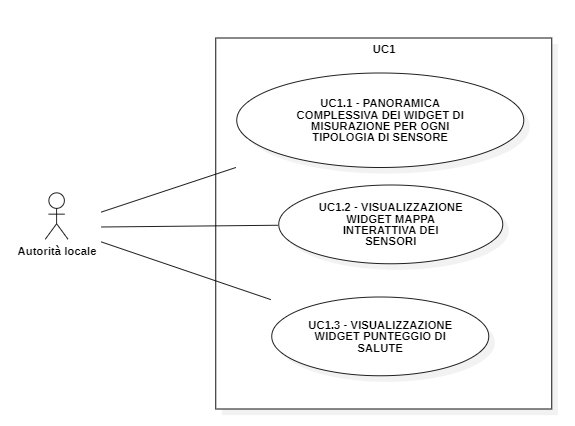
\includegraphics[width=0.9\textwidth]{../Images/uc1_Subcase.PNG} 
    \caption{Sottocasi UC1 - VISUALIZZAZIONE DASHBOARD}
    \label{fig:UC1_sub}
\end{figure}

%---------------------------- UC1.1 ---------------------------------

\subsubsection{UC1.1 - PANORAMICA COMPLESSIVA DEI WIDGET DI MISURAZIONE PER OGNI TIPOLOGIA DI SENSORE}
\begin{itemize}
    \item \textbf{Attore principale:} Autorità locale.
    \item \textbf{Descrizione:} L'autorità locale accede alla dashboard della città e visualizza un widget contente un grafico aggiornato in tempo reale, il quale rappresenta i dati registrati durante la giornata per ogni tipologia di sensore che trasmette al sistema.
    \item \textbf{Scenario principale:}
        \begin{enumerate}
            \item L'utente accede alla piattaforma per la visualizzazione della dashboard della città. (UC1)
            \item Il sistema elabora le informazioni ricevute dai sensori e imposta la visualizzazione di un widget con le misurazioni quotidiane per ogni tipolgia di sensore;
        \end{enumerate}
    \item \textbf{Precondizioni:}
        \begin{itemize}
            \item Nessuna
        \end{itemize}
    \item \textbf{Postcondizioni:}
        \begin{itemize}
            \item L'autorità locale ha una visione di un widget con misurazioni aggiornate in tempo reale, il quale rappresenta i dati registrati durante la giornata per ogni tipologia di sensore.
        \end{itemize}
    \item \textbf{User story associata:}
        \begin{itemize}
            \item Come autorità locale voglio visualizzare widget come le misurazioni aggiornate in tempo reale sui dati registrati durante la giornata per ogni tipologia di sensore nella dashboard.
        \end{itemize}
\end{itemize}


%---------------------------- UC1.2 ---------------------------------

\subsubsection{UC1.2 - Visualizzazione mappa sensori}
\begin{itemize}
    \item \textbf{Attore principale:} Autorità locale.
    \item \textbf{Descrizione:} L'autorità locale accede alla dashboard della città e visualizza una mappa con una visione dei sensori posizionati nella città.
    \item \textbf{Scenario principale:}
          \begin{enumerate}
              \item L'utente visualizza una mappa contenente i sensori nella corretta posizione. (i sensori sono etichettati per riconoscere la tipologia)
          \end{enumerate}
    \item \textbf{Precondizioni:}
          \begin{itemize}
              \item  Almeno un sensore è attivo e ha trasmesso dati;
              \item L'utente si trova nella dashboard della città. (UC1)
          \end{itemize}
    \item \textbf{Postcondizioni:}
          \begin{itemize}
              \item      L'utente ha una visione grafica aggiornata della mappa dei sensori nella città e della loro tipologia.
          \end{itemize}
    \item \textbf{User story associata:}
          \begin{itemize}
              \item Come autorità locale, voglio essere in grado di visualizzare una mappa contenente i sensori attivi e operativi all'interno della città. La mappa deve mostrare chiaramente la posizione di ciascun sensore e devono essere etichettati per consentire un riconoscimento immediato della tipologia di ogni sensore.
          \end{itemize}
\end{itemize}

%---------------------------- UC1.3 ---------------------------------
\newpage

\subsubsection{UC1.3 - VISUALIZZAZIONE WIDGET PUNTEGGIO DI SALUTE}
\begin{itemize}
    \item \textbf{Attore principale:} Autorità locale.
    \item \textbf{Precondizioni:}
        \begin{itemize}
            \item Il sistema è operativo e accessibile.
        \end{itemize}
    \item \textbf{Postcondizioni:}
        \begin{itemize}
            \item L'autorità locale ha una visione aggiornata di un punteggio, un numero intero, rappresentante lo stato di salute della città.
        \end{itemize}
    \item \textbf{Scenario principale:}
          \begin{enumerate}
            \item L'autorità locale accede alla piattaforma per la visualizzazione della dashboard. (UC1)
            \item Il sistema elabora i dati provenienti dai sensori e calcola un punteggio di salute.
        \end{enumerate}
    \item \textbf{User story associata:} \\
        Come autorità locale, desidero visualizzare un punteggio ottenuto tramite una funzione di aggregazione, il quale fornisca una visione immediata di eventuali dati anomali rilevati dai sensori disseminati nella città, al fine di identificare rapidamente situazioni critiche e prendere azioni tempestive per garantire la sicurezza e il benessere della comunità.
\end{itemize}

%---------------------------- SUB_UC1.1 ---------------------------------
\newpage

\begin{figure}[H]
    \centering
    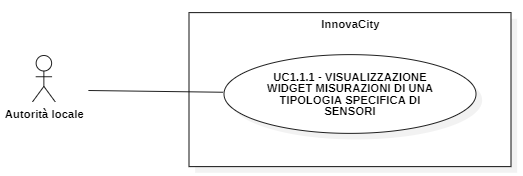
\includegraphics[width=0.9\textwidth]{../Images/uc1.1.1.png}
    \caption{UC1.1.1 - VISUALIZZAZIONE WIDGET MISURAZIONI DI UNA TIPOLOGIA SPECIFICA DI SENSORI}
    \label{fig:UC3}
\end{figure}

%---------------------------- UC1.1.1 ---------------------------------

\subsubsection{UC1.1.1 - VISUALIZZAZIONE WIDGET MISURAZIONI DI UNA TIPOLOGIA SPECIFICA DI SENSORI}

\begin{itemize}
    \item \textbf{Attore principale:} Autorità locale;
    \item \textbf{Precondizioni:}
        \begin{itemize}
            \item Il sistema è operativo e accessibile.
        \end{itemize}
    \item \textbf{Postcondizioni:}
        \begin{itemize}
            \item L'autorità locale visualizza uno specifico widget contenente le misurazioni rilevate da una specifica tipologia di sensori.
        \end{itemize}
    \item \textbf{Scenario principale:}
        \begin{enumerate}
            \item Il sistema ha caricato la visualizzazione della dashboard (UC1).
            \item Il sistema carica i dati e imposta la visualizzazione di uno specifico widget contenente le misurazioni relative ad una specifica tipologia di sensori.
        \end{enumerate}
    \item \textbf{User story associata:} \\
        Come autorità locale, voglio accedere a un widget dettagliato che rappresenti le misurazioni provenienti da una specifica tipologia di sensori. Questo mi permetterà di analizzare in modo approfondito i dati relativi a quella tipologia di sensori, aiutandomi a prendere decisioni mirate per migliorare i servizi della città.
\end{itemize}

%---------------------------- SUB_UC1.1.1 ---------------------------------

\begin{figure}[H]
    \centering
    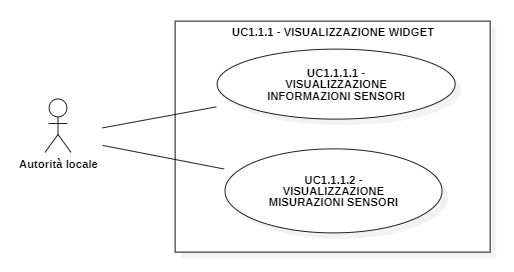
\includegraphics[width=0.9\textwidth]{../Images/subUC1.1.1.PNG}
    \caption{Sottocasi UC1.1.1 - VISUALIZZAZIONE WIDGET MISURAZIONI DI UNA TIPOLOGIA SPECIFICA DI SENSORI}
    \label{fig:UC3_sub}
\end{figure}

%---------------------------- UC1.1.1.1 ---------------------------------

\subsubsection{UC1.1.1.1 - VISUALIZZAZIONE INFORMAZIONI SENSORI}
\begin{itemize}
    \item \textbf{Attore principale:} Autorità locale;
    \item \textbf{Precondizioni:}
        \begin{itemize}
            \item Il \textit{sistema}\textsubscript{\textit{G}} è operativo e accessibile.
        \end{itemize}
    \item \textbf{Postcondizioni:}
        \begin{itemize}
            \item L’autorità locale ha una visione dettagliata sugli identificativi dei sensori che contribuiscono alle misurazioni rappresentate nel \textit{widget}\textsubscript{\textit{G}}.
        \end{itemize}
    \item \textbf{Scenario principale:}
        \begin{enumerate}
            \item Il \textit{sistema}\textsubscript{\textit{G}} carica e configura la visualizzazione di un \textit{widget}\textsubscript{\textit{G}} di una specifica tipologia di sensori (UC1.1.1);
            \item Il \textit{sistema}\textsubscript{\textit{G}} carica e configura la visualizzazione all'interno del \textit{widget}\textsubscript{\textit{G}} delle informazioni dei sensori coinvolti.
        \end{enumerate}
    \item \textbf{User story associata:} \\
        Come autorità locale, desidero visualizzare gli identificativi dei sensori associati alle misurazioni presentate nel \textit{widget}\textsubscript{\textit{G}}. Questo mi consentirà di comprendere meglio l'origine delle informazioni e facilitare la gestione e l'interpretazione dei dati raccolti.
\end{itemize}



%---------------------------- UC1.1.1.2 ---------------------------------

\subsubsection{UC1.1.1.2 - VISUALIZZAZIONE MISURAZIONI SENSORI}
\begin{itemize}
    \item \textbf{Attore principale:} Autorità locale;
    \item \textbf{Precondizioni:}
        \begin{itemize}
            \item Il \textit{sistema}\textsubscript{\textit{G}} è operativo e accessibile.
        \end{itemize}
    \item \textbf{Postcondizioni:}
        \begin{itemize}
            \item  L'autorità locale visualizza le misurazioni dei sensori associati al \textit{widget}\textsubscript{\textit{G}}.
        \end{itemize}
    \item \textbf{Scenario principale:}
        \begin{enumerate}
            \item Il \textit{sistema}\textsubscript{\textit{G}} carica e configura la visualizzazione di un \textit{widget}\textsubscript{\textit{G}} di una specifica tipologia di sensori (UC1.1.1);
            \item Il \textit{sistema}\textsubscript{\textit{G}} carica e configura la visualizzazione all'interno del \textit{widget}\textsubscript{\textit{G}} delle misurazioni dei sensori coinvolti.
        \end{enumerate}
    \item \textbf{User story associata:} \\
        Come autorità locale, desidero visualizzare le misurazioni dei sensori di una specifica tipologia per poter effettuare analisi mirate e prendere decisioni informate in base ai dati raccolti.
\end{itemize}


\begin{figure}[H]
    \centering
    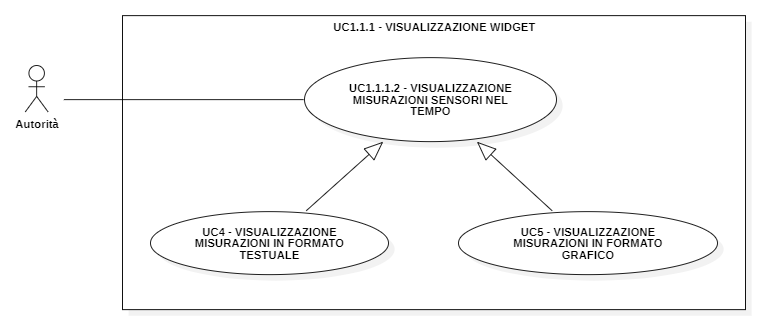
\includegraphics[width=0.9\textwidth]{../Images/uc1.1.1.2Gen.PNG}
    \caption{Generalizzazione UC1.1.1.2 - VISUALIZZAZIONE MISURAZIONI SENSORI}
    \label{fig:UC3_gen}
\end{figure}

\newpage

%---------------------------- UC4 ---------------------------------

\subsubsection{UC4 - Visualizzazione storico dati in formato testuale}
\begin{itemize}
    \item \textbf{Attore principale:} Autorità locale;
    \item \textbf{Descrizione:} L’autorità locale seleziona i/il sensore/i della quale vuole visionare lo storico dei dati e imposta la visulizzazione in formato testuale: (TIMESTAMP, Dato).
    \item \textbf{Scenario principale:}
          \begin{enumerate}
              \item L'utente imposta la visualizzazione in formato testuale.
          \end{enumerate}
    \item \textbf{Precondizioni:}
          \begin{itemize}
              \item  I/Il sensori/e di cui si vogliono visualizzare i dati storici ha trasmesso dati;
              \item  L'utente si trova in un interfaccia per la visualizzazione di uno storico dati (UC3).
          \end{itemize}
    \item \textbf{Postcondizioni:}
          \begin{itemize}
              \item  L'utente ha una visione dello storico dei dati trasmessi nel formato (TIMESTAMP, dato).
          \end{itemize}
    \item \textbf{User story associata:}
          \begin{itemize}
              \item Come autorità locale,
                    desidero visualizzare lo storico dei dati in formato testuale (TIMESTAMP, Dato),
                    In modo da avere una visione dettagliata delle informazioni trasmesse dai sensori.
          \end{itemize}
\end{itemize}

%---------------------------- UC5 ---------------------------------

\subsubsection{UC5 - VISUALIZZAZIONE MISURAZIONI IN FORMATO GRAFICO \newline TIME SERIES}
\begin{itemize}
    \item \textbf{Attore principale:} Autorità locale;
    \item \textbf{Precondizioni:}
        \begin{itemize}
            \item Il sistema è operativo e accessibile.
        \end{itemize}
    \item \textbf{Postcondizioni:}
        \begin{itemize}
            \item L'utente visualizza le misurazioni associate al widget attraverso un grafico time series.
        \end{itemize}
    \vspace{1cm}
    \item \textbf{Scenario principale:}
        \begin{enumerate}
            \item Il sistema carica e configura la visualizzazione di un widget di una specifica tipologia di sensori (UC1.1.1);
                \item Il sistema carica e configura la visualizzazione all'interno del widget delle misurazioni dei sensori coinvolti;
                \item L'autorità locale seleziona la visualizzazione delle misurazioni associato al widget in formato grafico.
        \end{enumerate}
    \item \textbf{User story associata:} \\
        Come autorità locale, desidero visualizzare le misurazioni associate ad uno specifico widget attraverso un grafico time series. Questo consente di semplificare la comprensione e la comparazione delle misurazioni, permettendo di individuare tendenze, relazioni e pattern in modo chiaro e rapido.
\end{itemize}
%---------------------------- UC14 ---------------------------------

\subsubsection{UC14 - VISUALIZZAZIONE MISURAZIONI IN FORMATO MAPPA INTERATTIVA}
\begin{itemize}
    \item \textbf{Attore principale:} Autorità locale;
    \item \textbf{Precondizioni:}
        \begin{itemize}
            \item Il sistema è operativo e accessibile.
        \end{itemize}
    \item \textbf{Postcondizioni:}
        \begin{itemize}
            \item L'utente visualizza le misurazioni correlate al widget mediante una mappa interattiva, la quale espone, attraverso apposite etichette, l'ultima rilevazione effettuata da ciascun sensore sulla mappa.
        \end{itemize}
    \item \textbf{Scenario principale:}
        \begin{enumerate}
            \item Il sistema carica e configura la visualizzazione di un widget di una specifica tipologia di sensori (UC1.1.1);
                \item Il sistema carica e configura la visualizzazione all'interno del widget delle misurazioni dei sensori coinvolti;
                \item Il widget è associato a sensori che generano dati binari (ex. Occupato / Libero, In funzione / Guasto).
              %  \item L'autorità locale seleziona la visualizzazione delle misurazioni associato al widget in formato mappa interattiva.
        \end{enumerate}
    \item \textbf{User story associata:} \\
        Come autorità locale, desidero poter visualizzare in modo chiaro e intuitivo le ultime rilevazioni effettuate da ciascun sensore associato al widget tramite una mappa interattiva, la quale, mediante etichette appropriate, rappresenti il valore della ultima misurazione effettuata da ciascun sensore.
\end{itemize}

%---------------------------- UC2 ---------------------------------
\begin{figure}[H]
    \centering
    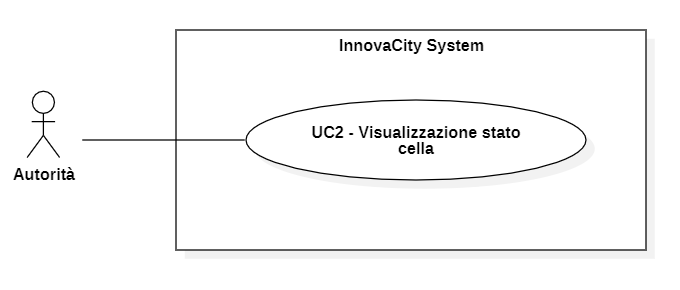
\includegraphics[width=0.9\textwidth]{../Images/uc2.png}
    \caption{UC2 - FILTRO VISUALIZZAZIONE DASHBOARD CELLA}
    \label{fig:UC2}
\end{figure}

\subsubsection{UC2 - Visualizzazione stato cella}
\begin{itemize}
    \item \textbf{Attore principale:} Autorità locale.
    \item \textbf{Descrizione:} L'autorità locale effettua la selezione della cella, ossia la specifica zona urbana, al fine di visualizzare in tempo reale i dati provenienti da varie tipologie di sensori ubicati nella suddetta area. Ciò permette una valutazione reapida dello stato complessivo della cella.
    \item \textbf{Scenario principale:}
        \begin{enumerate}
            \item L'utente seleziona la cella per la quale desidera visualizzare la dashboard contenente esclusivamente i dati correlati a essa.
        \end{enumerate}
    \item \textbf{Precondizioni:}
        \begin{itemize}
            \item  Almeno un sensore presente nella cella ha trasmesso dati;
            \item L'utente si trova  nella piattaforma per la visualizzazione della dashboard sullo stato della città (UC1);
        \end{itemize}
    \item \textbf{Postcondizioni:}
        \begin{itemize}
            \item  L'utente ha una visione aggiornata dello stato di salute della cella tramite widget e grafici interattivi aggiornati in tempo reale sulla base di dati correlati esclusivamente alla cella, inoltre visualizza una mappa dei sensori presenti nella cella e un punteggio di salute relativo alla cella.
          \end{itemize}
    \item \textbf{User story associata:}
        \begin{itemize}
            \item Come autorità locale, desidero poter selezionare una specifica cella urbana sulla piattaforma al fine di visualizzare immediatamente i dati provenienti da vari sensori presenti nell'area. Questo mi permetterà di valutare rapidamente lo stato complessivo della cella e prendere decisioni informate.
        \end{itemize}
\end{itemize}

%---------------------------- UC6 ---------------------------------

\begin{figure}[H]
    \centering
    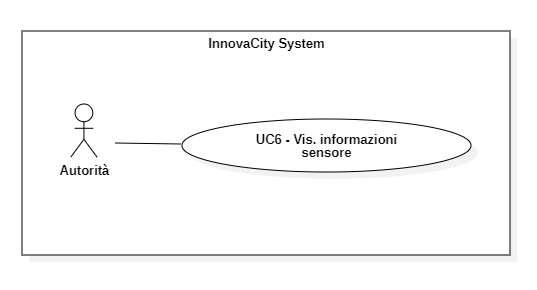
\includegraphics[width=0.9\textwidth]{../Images/uc6.png}
    \caption{UC6 - VISUALIZZAZIONE WIDGET SENSORI TEMPERATURA}
    \label{fig:UC6}
\end{figure}

\subsubsection{UC6 - VISUALIZZAZIONE WIDGET SENSORI TEMPERATURA}
\begin{itemize}
    \item \textbf{Attore principale:} Autorità locale;
    \item \textbf{Precondizioni:}
        \begin{itemize}
            \item Almeno un sensore di temperatura ha trasmesso dati al sistema;
            \item Il sistema ha caricato la visualizzazione della dashboard (UC1).
        \end{itemize}
    \item \textbf{Postcondizioni:}
        \begin{itemize}
            \item L'autorità locale visualizza un widget contenente le misurazioni relative ai sensori di temperatura.
        \end{itemize}
    \item \textbf{Scenario principale:}
        \begin{enumerate}
            \item Il sistema carica i dati e imposta la visualizzazione del widget contenente le misurazioni relative ai sensori di temperatura.
        \end{enumerate}
    \item \textbf{User story associata:} \\
        Come autorità locale, desidero visualizzare un widget per la visualizzazione delle misurazioni trasmesse dai sensori di temperatura. Questo mi permetterà di analizzare in modo approfondito i dati relativi a quella tipologia di sensori, aiutandomi a prendere decisioni mirate per migliorare i servizi della città.
\end{itemize}

%---------------------------- UC7 ---------------------------------

\begin{figure}[H]
    \centering
    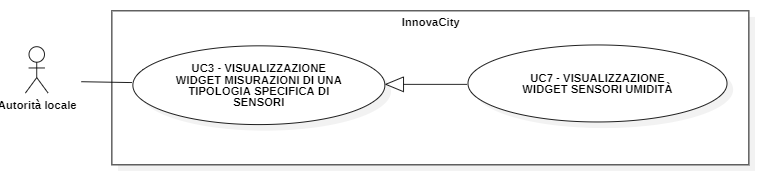
\includegraphics[width=0.9\textwidth]{../Images/uc7.png}
    \caption{UC7 - VISUALIZZAZIONE WIDGET SENSORI UMIDITÀ}
\end{figure}

\subsubsection{UC7 - VISUALIZZAZIONE WIDGET SENSORI UMIDITÀ}
\begin{itemize}
    \item \textbf{Attore principale:} Autorità locale;
    \item \textbf{Precondizioni:}
        \begin{itemize}
            \item Il sistema ha caricato la visualizzazione della dashboard (UC1).
        \end{itemize}
    \item \textbf{Postcondizioni:}
        \begin{itemize}
            \item L'autorità locale visualizza un widget contenente le misurazioni relative ai sensori di umidità.
        \end{itemize}
    \item \textbf{Scenario principale:}
        \begin{enumerate}
            \item Il sistema carica i dati e imposta la visualizzazione del widget contenente le misurazioni relative ai sensori di umidità.
        \end{enumerate}
    \item \textbf{User story associata:} \\
        Come autorità locale, desidero visualizzare un widget per la visualizzazione delle misurazioni trasmesse dai sensori di umidità. Questo mi permetterà di analizzare in modo approfondito i dati relativi a quella tipologia di sensori, aiutandomi a prendere decisioni mirate per migliorare i servizi della città.
\end{itemize}

%---------------------------- UC8 ---------------------------------

\begin{figure}[H]
    \centering
    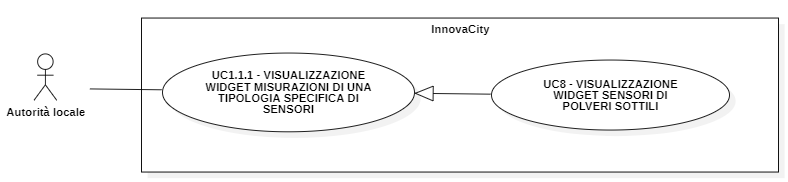
\includegraphics[width=0.9\textwidth]{../Images/uc8.PNG}
    \caption{UC8 - VISUALIZZAZIONE WIDGET SENSORI DI POLVERI SOTTILI}
\end{figure}

\subsubsection{UC8 - VISUALIZZAZIONE WIDGET SENSORI DI POLVERI SOTTILI}
\begin{itemize}
    \item \textbf{Attore principale:} Autorità locale;
    %\item \textbf{Descrizione:} L’autorità locale dalla pagina adibita alla visione dello storico dati di un sensore seleziona la visualizzazione delle informazioni sul sensore.
    \item \textbf{Scenario principale:}
          \begin{enumerate}
              \item L'autorità locale seleziona la visualizzazione del widget dei sensori di polveri sottili.
          \end{enumerate}
    \item \textbf{Precondizioni:}
          \begin{itemize}
              \item  Almeno un sensore di polveri sottili ha trasmesso dati al sistema.
          \end{itemize}
    \item \textbf{Postcondizioni:}
          \begin{itemize}
              \item  L'autorità locale ha una visione di un widget contenente le informazioni dei sensori di polveri sottili.
          \end{itemize}
    \item \textbf{User story associata:}
          \begin{itemize}
              \item Come Autorità locale, desidero visualizzare un widget per la visualizzazione delle misurazione dei sensori di polveri sottili.
          \end{itemize}
\end{itemize}

%---------------------------- UC9 ---------------------------------
\begin{figure}[H]
    \centering
    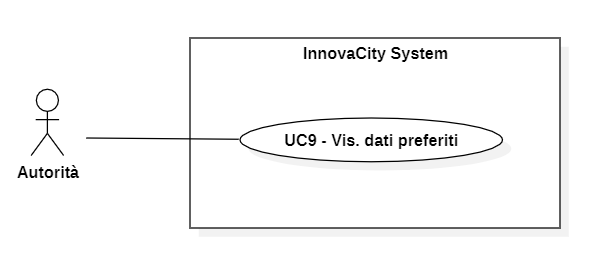
\includegraphics[width=0.9\textwidth]{../Images/uc9.png}
    \caption{UC9 - VISUALIZZAZIONE WIDGET SENSORI DI GUASTI ELETTRICI}
\end{figure}

\subsubsection{UC9 - Visualizzazione dati preferiti}
\begin{itemize}
    \item \textbf{Attore principale:} Autorità locale;
    \item \textbf{Descrizione:} L’autorità locale seleziona la visulizzazione dei dati preferiti.
    \item \textbf{Scenario principale:}
          \begin{enumerate}
              \item L'utente accede alla piattaforma per la visualizzazione della dashboard sullo stato della città o di una cella(UC1) (UC1.1);
              \item L'utente sceglie di visualizzare la pagina dedicata alla visualizzazione dei dati preferiti.
          \end{enumerate}
    \item \textbf{Precondizioni:}
          \begin{itemize}
              \item  L'utente si trova nella pagina per la visualizzazione delle dashboard (UC1) (UC1.1);
          \end{itemize}
    \item \textbf{Postcondizioni:}
          \begin{itemize}
              \item  L'utente ha una visione dei dati dei sensori salvati come preferiti.
          \end{itemize}
    \item \textbf{User story associata:}
          \begin{itemize}
              \item Come di Autorità Locale, desidero visualizzare i dati dei sensori precedentemente salvati come preferiti sulla piattaforma, così da poter accedere rapidamente alle informazioni rilevanti.
          \end{itemize}
\end{itemize}
%---------------------------- UC10 ---------------------------------
\newpage

\begin{figure}[H]
    \centering
    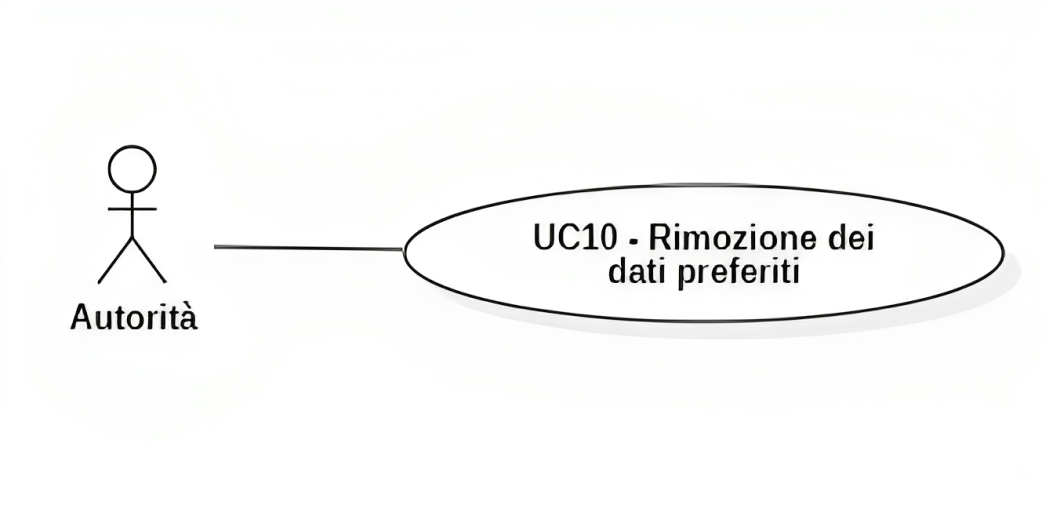
\includegraphics[width=0.9\textwidth]{../Images/uc10.png}
    \caption{UC10 - VISUALIZZAZIONE WIDGET SENSORI ISOLE ECOLOGICHE}
\end{figure}

\subsubsection{UC10 - VISUALIZZAZIONE WIDGET SENSORI ISOLE ECOLOGICHE}
\begin{itemize}
    \item \textbf{Attore principale:} Autorità locale;
    \item \textbf{Precondizioni:}
        \begin{itemize}
            \item Almeno un sensore di rilevamento soglia delle isole ecologiche ha trasmesso dati al sistema;
            \item Il sistema ha caricato la visualizzazione della dashboard (UC1).
        \end{itemize}
    \item \textbf{Postcondizioni:}
        \begin{itemize}
            \item L'autorità locale visualizza un widget contenente le misurazioni relative ai sensori di rilevamento soglia delle isole ecologiche.
        \end{itemize}
    \item \textbf{Scenario principale:}
        \begin{enumerate}
            \item Il sistema carica i dati e imposta la visualizzazione del widget contenente le misurazioni relative ai sensori di rilevamento soglia delle isole ecologiche.
        \end{enumerate}
    \item \textbf{User story associata:} \\
        Come autorità locale, desidero visualizzare un widget per la visualizzazione delle misurazioni trasmesse dai sensori di rilevamento soglia delle isole ecologiche. Questo mi permetterà di analizzare in modo approfondito i dati relativi a quella tipologia di sensori, aiutandomi a prendere decisioni mirate per migliorare i servizi della città.
\end{itemize}
%---------------------------- UC11 ---------------------------------
\begin{figure}[H]
    \centering
    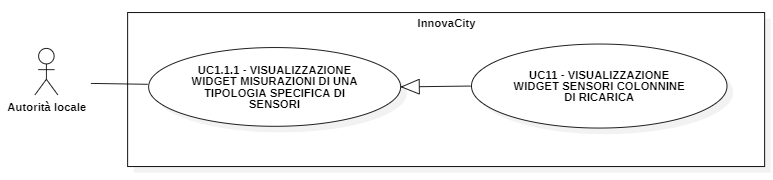
\includegraphics[width=0.9\textwidth]{../Images/uc11.PNG}
    \caption{UC11 - VISUALIZZAZIONE WIDGET SENSORI COLONNINE DI RICARICA}
\end{figure}

\subsubsection{UC11 - Visualizzazione storico dati in ordine crescente}
\begin{itemize}
    \item \textbf{Attore principale:} Autorità locale;
    \item \textbf{Descrizione:} L’autorità locale seleziona i/il sensore/i della quale vuole visionare lo storico dei dati in formato testuale in ordine crescente rispetto alle misurazioni del/i sensore/i.
    \item \textbf{Scenario principale:}
          \begin{enumerate}
              \item L'utente imposta la visualizzazione in ordine crescente.
          \end{enumerate}
    \item \textbf{Precondizioni:}
          \begin{itemize}
              \item  I/Il sensori/e di cui si vuole visualizzare i dati storici ha trasmesso dati;
              \item  L'utente si trova in un interfaccia per la visualizzazione di uno storico dati (UC3);
              \item La visualizzazione è impostata nel formato testuale (UC4);
          \end{itemize}
    \item \textbf{Postcondizioni:}
          \begin{itemize}
              \item  L'utente ha una visione dello storico dei dati trasmessi nel formato (TIMESTAMP, dato) in ordine crescente rispetto alle misurazioni.
          \end{itemize}
    \item \textbf{User story associata:}
          \begin{itemize}
              \item Come autorità locale, desidero essere in grado di visualizzare lo storico dei dati provenienti dai sensori in formato testuale, ordinati in modo crescente rispetto alla misurazione del/i sensore/i, al fine di identificare facilmente tendenze, cambiamenti o pattern nel tempo.
          \end{itemize}
\end{itemize}

%---------------------------- UC33 ---------------------------------

\begin{figure}[H]
    \centering
    \includegraphics[width=0.9\textwidth]{../Images/uc33.PNG}
    \caption{UC33 - VISUALIZZAZIONE WIDGET SENSORI LIVELLO DELL'ACQUA}
\end{figure}

\subsubsection{UC33 - VISUALIZZAZIONE WIDGET SENSORI LIVELLO DELL'ACQUA}
\begin{itemize}
    \item \textbf{Attore principale:} Autorità locale;
    \item \textbf{Precondizioni:}
        \begin{itemize}
            \item Almeno un sensore del livello dell'acqua ha trasmesso dati al sistema;
            \item Il sistema ha caricato la visualizzazione della dashboard (UC1).
        \end{itemize}
    \item \textbf{Postcondizioni:}
        \begin{itemize}
            \item L'autorità locale visualizza un widget contenente le misurazioni relative ai sensori del livello dell'acqua.
        \end{itemize}
    \item \textbf{Scenario principale:}
        \begin{enumerate}
            \item Il sistema carica i dati e imposta la visualizzazione del widget contenente le misurazioni relative ai sensori del livello dell'acqua.
        \end{enumerate}
    \item \textbf{User story associata:} \\
        Come autorità locale, desidero visualizzare un widget per la visualizzazione delle misurazioni trasmesse dai sensori del livello dell'acqua. Questo mi permetterà di analizzare in modo approfondito i dati relativi a quella tipologia di sensori, aiutandomi a prendere decisioni mirate per migliorare i servizi della città.
\end{itemize}

%---------------------------- UC12 ---------------------------------
\newpage

\begin{figure}[H]
    \centering
    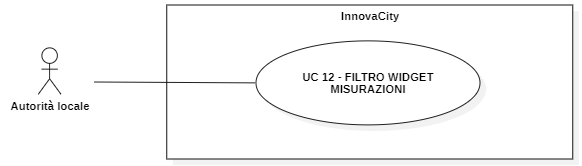
\includegraphics[width=0.9\textwidth]{../Images/uc12.PNG}
    \caption{UC 12 - FILTRO WIDGET MISURAZIONI}
\end{figure}

\subsubsection{UC12 - FILTRO WIDGET MISURAZIONI}
\begin{itemize}
    \item \textbf{Attore principale:} Autorità locale;
    \item \textbf{Precondizioni:}
        \begin{itemize}
            \item L'autorità locale si trova nell'interfaccia di visualizzazione di un \textit{widget}\textsubscript{\textit{G}} associato ad una specifica tipologia di sensori (UC1.1.1);
        \end{itemize}
    \item \textbf{Postcondizioni:}
          \begin{itemize}
              \item L'autorità locale visualizza esclusivamente le misurazioni che soddisfano il filtraggio.
          \end{itemize}
    \item \textbf{Scenario principale:}
          \begin{enumerate}
              \item L'utente seleziona i filtri da applicare;
              \item Il \textit{sistema}\textsubscript{\textit{G}} aggiorna la visualizzazione mostrando esclusivamente le misurazioni che rispettano i vincoli specificati filtri.
          \end{enumerate}
    \item \textbf{User story associata:} \\
        Come autorità locale, desidero disporre della capacità di applicare filtri per la visualizzazione delle misurazioni, consentendo un'analisi dettagliata e focalizzata attraverso una combinazione di criteri selettivi.
\end{itemize}


%---------------------------- UC12.1 ---------------------------------
\newpage

\begin{figure}[H]
    \centering
    \includegraphics[width=0.9\textwidth]{../Images/uc12.1.PNG}
    \caption{UC12.1 - FILTRO VISUALIZZAZIONE MISURAZIONI IN UN INTERVALLO TEMPORALE}
\end{figure}

\subsubsection{UC12.1 - FILTRO VISUALIZZAZIONE MISURAZIONI IN UN INTERVALLO TEMPORALE}
\begin{itemize}
    \item \textbf{Attore principale:} Autorità locale;
    \item \textbf{Precondizioni:}
        \begin{itemize}
            \item L'autorità locale si trova nell'interfaccia di visualizzazione di un \textit{widget}\textsubscript{\textit{G}} associato ad una specifica tipologia di sensori (UC1.1.1); 
            \item L'autorità locale ha impostato la vista in formato testuale time series o in formato grafico time series.
        \end{itemize}
    \item \textbf{Postcondizioni:}
        \begin{itemize}
            \item L'autorità locale visualizza le sole misurazioni trasmesse da una specifica tipolgia di sensori nell'intervallo temporale selezionato.
        \end{itemize}
    \item \textbf{Scenario principale:}
        \begin{enumerate}
            \item L'autorità locale seleziona la funzionalità relativa al filtro dei dati per intervallo temporale;
            \item L'autorità locale imposta un intervallo temporale;
            \item Il \textit{sistema}\textsubscript{\textit{G}} verifica la validità dell'intervallo temporale inserito;
            \item Il \textit{sistema}\textsubscript{\textit{G}} aggiorna la visualizzazione mostrando solo le misurazioni effettuate durante l'intervallo temporale. selezionato.
        \end{enumerate}
    \item \textbf{Estensioni:}
    \begin{enumerate}
        \item VISUALIZZAZIONE ERRORE INTERVALLO TEMPORALE NON VALIDO (UC30)
    \end{enumerate}
    \item \textbf{User story associata:} \\
        Come autorità locale, voglio avere la capacità di definire un intervallo temporale personalizzato per poter filtrare le misurazioni trasmesse da una specifica tipologia di sensori. Ciò mi permetterà di analizzare dettagliatamente le misurazioni raccolte in un periodo di interesse specifico.
\end{itemize}

%---------------------------- UC30 ---------------------------------
\subsubsection{UC30 - VISUALIZZAZIONE ERRORE INTERVALLO TEMPORALE NON VALIDO}
\begin{itemize}
      \item \textbf{Attore principale:} Autorità locale;
      \item \textbf{Precondizioni:}
            \begin{itemize} 
                  \item L'autorità locale specifica un intervallo temporale non valido per la visualizzazione filtrata delle misurazioni;
            \end{itemize}
            \item \textbf{Postcondizioni:}
            \begin{itemize}
                  \item L'autorità locale visualizza un messaggio di errore.
            \end{itemize}
            \item \textbf{Scenario principale:}
            \begin{enumerate}
                  \item Il sistema rileva l'invalidità dell'intervallo temporale specificato dall'autorità locale.
                  \end{enumerate}
      \item \textbf{User story associata:} \\
            Come autorità locale, desidero ricevere una notifica immediata nel caso in cui selezioni un intervallo temporale non valido come filtro per la visualizzazione delle misurazioni. Questo mi permetterà di ricevere un feedback istantaneo e mi darà la possibilità di inserire successivamente un intervallo temporale corretto.
\end{itemize}

%---------------------------- UC12.2 ---------------------------------

\begin{figure}[H]
    \centering
    \includegraphics[width=0.9\textwidth]{../Images/uc12.2.PNG}
    \caption{UC12.2 -FILTRO VISUALIZZAZIONE PER MISURAZIONI}
\end{figure}

\subsubsection{UC12.2 - FILTRO VISUALIZZAZIONE PER MISURAZIONI}
\begin{itemize}
    \item \textbf{Attore principale:} Autorità locale;
    \item \textbf{Precondizioni:}
        \begin{itemize}
            \item L'autorità locale si trova nell'interfaccia di visualizzazione di un widget associato ad una specifica tipologia di sensori (UC1.1.1);
            \item L'autorità locale ha impostato la vista in formato testuale Time series o in formato grafico Time Series.
        \end{itemize}
    \item \textbf{Postcondizioni:}
        \begin{itemize}
            \item L'utente visualizza le misurazioni filtrate includendo soltanto i dati rilevati che si collocano tra i due valori specificati.
        \end{itemize}
    \item \textbf{Scenario principale:}
        \begin{enumerate}
            \item L'autorità locale seleziona la funzionalità relativa al filtro dei dati per intervallo di rilevamento;
            \item L'utente inserisce un valore di minimo ed un valore di massimo per filtrare le misurazioni;
            \item Il sistema verifica la validità dell'intervallo di rilevamento inserito;
            \item Il sistema aggiorna la visualizzazione mostrando esclusivamente le misurazioni con il dato rilevato che ricade all'interno dell'intervallo specificato.
        \end{enumerate}
    \item \textbf{Estensioni:}
        \begin{enumerate}
            \item VISUALIZZAZIONE ERRORE INTERVALLO DI RILEVAMENTO NON VALIDO (UC32)
        \end{enumerate}
    \item \textbf{User story associata:} \\
        Come autorità locale, desidero avere la possibilità di visualizzare le misurazioni filtrate includendo soltanto i dati rilevati che si collocano tra un valore di minimo e di massimo specifici. Questo mi consentirà di analizzare in modo più mirato e focalizzato le misurazioni che rientrano in un determinato intervallo di rilevamento, facilitando l'identificazione di pattern o anomalie significative.
\end{itemize}


%---------------------------- UC32 ---------------------------------
\subsubsection{UC30 - VISUALIZZAZIONE ERRORE INTERVALLO DI RILEVAMENTO NON VALIDO}
\begin{itemize}
    \item \textbf{Attore principale:} Autorità locale;
    \item \textbf{Precondizioni:}
        \begin{itemize} 
            \item L'autorità locale specifica un intervallo di rilevamento non valido per la visualizzazione filtrata delle misurazioni;
            \item Il sistema rileva l'invalidità dell'intervallo di rilevamento specificato dall'autorità locale.
        \end{itemize}
    \item \textbf{Postcondizioni:}
        \begin{itemize}
            \item L'autorità locale visualizza un messaggio di errore e viene richiesto l'inserimento di un nuovo intervallo di rilevamento.
        \end{itemize}
    \item \textbf{Scenario principale:}
            \begin{enumerate}
            \item L'autorità locale visualizza di un messaggio di errore;
            \item Il sistema richiede all'autorità locale di inserire un intervallo di rilevamento valido.
            \end{enumerate}
    \item \textbf{User story associata:}
        Come autorità locale, desidero ricevere una notifica immediata nel caso in cui selezioni un intervallo di rilevamento non valido come filtro per la visualizzazione delle misurazioni. Questo mi permetterà di ricevere un feedback istantaneo e mi darà la possibilità di inserire successivamente un intervallo di rilevamento corretto.
\end{itemize}

%---------------------------- UC12.3 ---------------------------------
\newpage

\begin{figure}[H]
    \centering
    \includegraphics[width=0.9\textwidth]{../Images/uc12.3.PNG}
    \caption{UC12.3 - FILTRO VISUALIZZAZIONE MISURAZIONI PER CELLA}
\end{figure}

\subsubsection{UC12.3 - FILTRO VISUALIZZAZIONE MISURAZIONI PER CELLA}
\begin{itemize}
    \item \textbf{Attore principale:} Autorità locale;
    \item \textbf{Precondizioni:}
        \begin{itemize}
            \item L'autorità locale si trova nell'interfaccia di visualizzazione di un widget associato ad una specifica tipologia di sensori (UC1.1.1);
            \item Almeno una cella urbana è presente nella città. 
        \end{itemize}
    \item \textbf{Postcondizioni:}
          \begin{itemize}
              \item L'autorità locale visualizza esclusivamente le misurazioni trasmesse dai sensori di una o più specifiche celle selezionate.
          \end{itemize}
    \item \textbf{Scenario principale:}
          \begin{enumerate}
              \item L'autorità locale seleziona la funzionalità relativa al filtro per cella urbana;
              \item L'autorità locale seleziona una o più celle come filtro;
              \item Il sistema aggiorna la visualizzazione mostrando esclusivamente le misurazioni dei sensori all'interno delle celle urbane selezionate.
          \end{enumerate}
    \item \textbf{User story associata:} \\
        Come autorità locale, desidero poter filtrare la visualizzazione delle misurazioni in base alle singole celle urbane, consentendo un'esplorazione dettagliata dei dati rilevanti per ciascuna area della città.
\end{itemize}

%---------------------------- UC12.4 ---------------------------------
\begin{figure}[H]
    \centering
    \includegraphics[width=0.9\textwidth]{../Images/uc12.4.PNG}
    \caption{UC12.4 - FILTRO VISUALIZZAZIONE MISURAZIONI PER SENSORE}
\end{figure}
\subsubsection{UC12.4 - FILTRO VISUALIZZAZIONE MISURAZIONI PER SENSORE}
\begin{itemize}
    \item \textbf{Attore principale:} Autorità locale;
    \item \textbf{Precondizioni:}
        \begin{itemize}
            \item L'autorità locale si trova nell'interfaccia di visualizzazione di un widget associato ad una specifica tipologia di sensori (UC1.1.1);
        \end{itemize}
    \item \textbf{Postcondizioni:}
        \begin{itemize}
            \item L'autorità locale visualizza esclusivamente le misurazioni trasmesse da uno o più specifici sensori selezionati.
        \end{itemize}
    \item \textbf{Scenario principale:}
        \begin{enumerate}
            \item L'autorità locale seleziona la funzionalità relativa al filtro per sensore;
            \item L'autorità locale seleziona uno o più sensori come filtro;
            \item Il sistema aggiorna la visualizzazione mostrando esclusivamente le misurazioni tramsesse dai sensori selezionati.
        \end{enumerate}
    \item \textbf{User story associata:} \\
        Come autorità locale, desidero filtrare la visualizzazione delle misurazioni in base ad una selezione di specifici sensori, permettendo un'analisi dettagliata e specifica per ciascun sensore presenti nella città.
\end{itemize}


%---------------------------- UC13 ---------------------------------

\begin{figure}[H]
    \centering
    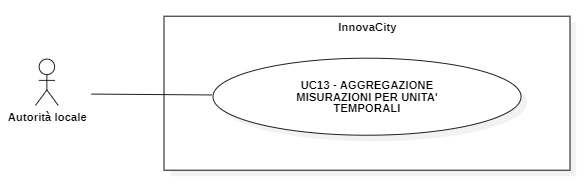
\includegraphics[width=0.9\textwidth]{../Images/uc13.PNG}
    \caption{UC13 - AGGREGAZIONE MISURAZIONI PER UNITA' TEMPORALI}
\end{figure}

\subsubsection{UC13 - Visualizzazione storico dati filtrato sulle misurazioni}
\begin{itemize}
    \item \textbf{Attore principale:} Autorità locale;
    \item \textbf{Descrizione:} L’autorità locale seleziona i/il sensore/i della quale vuole visionare lo storico dei dati e filtra la visualizzazione ai soli dati compresi tra due valori.
    \item \textbf{Scenario principale:}
          \begin{enumerate}
              \item L'utente configura due valori specifici al fine di visualizzare esclusivamente le misurazioni che ricadono all'interno di tale intervallo.
          \end{enumerate}
    \item \textbf{Precondizioni:}
          \begin{itemize}
              \item  I/Il sensori/e di cui si vuole visualizzare i dati storici ha trasmesso dati;
              \item  L'utente si trova in un interfaccia per la visualizzazione di uno storico dati (UC3).
          \end{itemize}
    \item \textbf{Postcondizioni:}
          \begin{itemize}
              \item  L'utente accede a una rappresentazione dello storico dei dati trasmessi, la cui visualizzazione è stata filtrata esclusivamente per includere le misurazioni con il dato compreso tra i due valori specificati.
          \end{itemize}
    \item \textbf{User story associata:}
          \begin{itemize}
            \item Come autorità locale, desidero avere la possibilità di filtrare la visualizzazione dello storico dei dati in base alle misurazioni del sensore comprese tra due valori specifici. Questo mi consentirà di analizzare in modo più mirato e focalizzato i dati che rientrano in un determinato intervallo, facilitando l'identificazione di pattern o anomalie significative.
          \end{itemize}
\end{itemize}


%---------------------------- UC31 ---------------------------------

\begin{figure}[H]
    \centering
    \includegraphics[width=0.9\textwidth]{../Images/uc31.PNG}
    \caption{UC31 - RIMOZIONE FILTRI}
    \label{fig:UC7}
\end{figure}
\subsubsection{UC31 - RIMOZIONE FILTRI}
\begin{itemize}
    \item \textbf{Attore principale:} Autorità locale;
    \item \textbf{Precondizioni:}
        \begin{itemize}
        \item L'autorità locale si trova nell'interfaccia di visualizzazione di un widget associato ad una specifica tipologia di sensori (UC1.1.1);
        \item La visualizzazione delle misurazioni include almeno un filtro attivo.
        \end{itemize}
    \item \textbf{Postcondizioni:}
        \begin{itemize}
            \item L'autorità locale visualizza le misurazioni senza nessun filtro applicato.
        \end{itemize}
    \item \textbf{Scenario principale:}
        \begin{enumerate}
            \item L'utente rimuove uno o più filtri relativi alle misurazioni.
            \item Il sistema aggiorna la visualizzazione senza l'applicazione dei filtri disattivati.
        \end{enumerate}
    \item \textbf{User story associata:} \\
        Come autorità locale, desidero rimuovere eventuali filtri attivi nella visualizzazione delle misurazioni in modo tale da tornare alla visualizzazione delle misurazioni senza tali filtri.
\end{itemize}


%---------------------------- UC18 ---------------------------------

\begin{figure}[H]
    \centering
    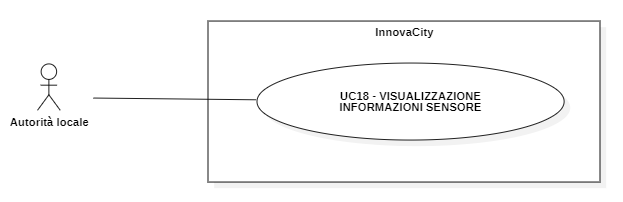
\includegraphics[width=0.9\textwidth]{../Images/uc18.PNG}
    \caption{UC18 - VISUALIZZAZIONE INFORMAZIONI SENSORE}
\end{figure}
\subsubsection{UC18 - VISUALIZZAZIONE INFORMAZIONI SENSORE}
\begin{itemize}
    \item \textbf{Attore principale:} Autorità locale;
    \item \textbf{Precondizioni:}
        \begin{itemize}
            \item Il sistema ha caricato la visualizzazione della dashboard (UC1);
        \end{itemize}
    \item \textbf{Postcondizioni:}
        \begin{itemize}
            \item L'autorità locale visualizza le informazioni relative ad uno specifico sensore.
        \end{itemize}
    \item \textbf{Scenario principale:}
        \begin{enumerate}
            \item L'autorità locale seleziona un sensore dalla mappa interattiva della città presente nella dashboard;
            \item Il sistema carica le informazioni relative al sensore selezionato.
        \end{enumerate}
    \item \textbf{User story associata:} \\
        Come autorità locale, desidero accedere alle informazioni dettagliate di un sensore specifico per ottenere una comprensione esaustiva delle sue caratteristiche e specifiche.
\end{itemize}

%---------------------------- SUB_UC18 ---------------------------------

\begin{figure}[H]
    \centering
    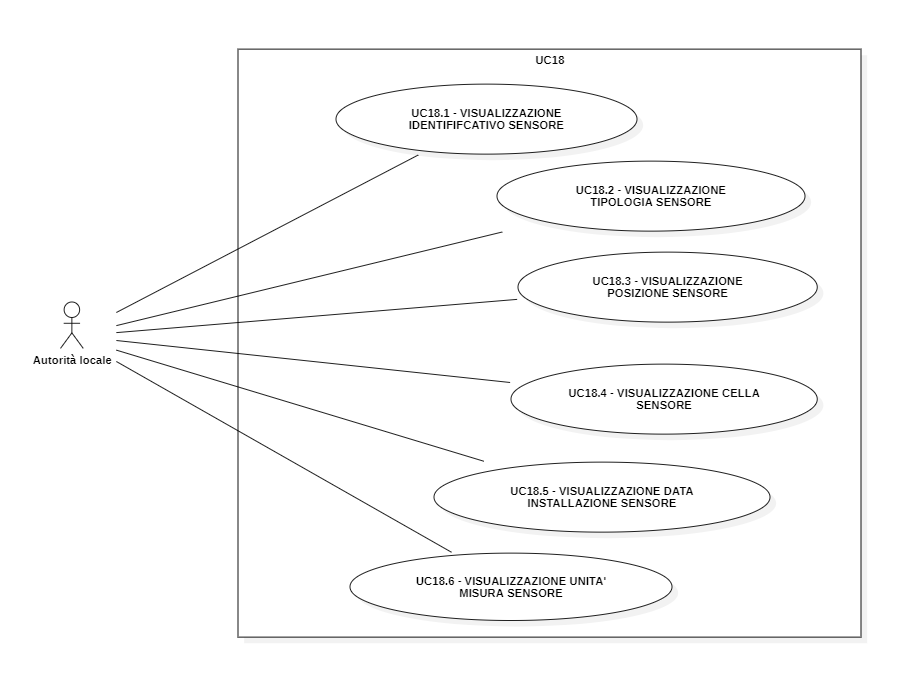
\includegraphics[width=0.9\textwidth]{../Images/uc18sub.PNG}
    \caption{SOTTOCASI UC18 - VISUALIZZAZIONE INFORMAZIONI SENSORE}
\end{figure}

%---------------------------- UC18.1 ---------------------------------

\subsubsection{UC18.1 - VISUALIZZAZIONE IDENTIFICATIVO SENSORE}
\begin{itemize}
    \item \textbf{Attore principale:} Autorità locale;
    %\item \textbf{Descrizione:} L’autorità locale dalla pagina adibita alla visione delle informazioni di un sensore visualizza il suo Identificativo.
    \item \textbf{Scenario principale:}
    \begin{enumerate}
        \item L'utente seleziona la visualizzazione delle informazioni del sensore.
    \end{enumerate}
\item \textbf{Precondizioni:}
    \begin{itemize}
        \item  L'utente di trova nella pagina di visualizzazione dello storico dei dati di un sensore. (3.3)
    \end{itemize}
    \item \textbf{Postcondizioni:}
          \begin{itemize}
              \item  L'utente visualizza l'Identificativo del sensore.
          \end{itemize}\item \textbf{User story associata:}
          \begin{itemize}
              \item Come Autorità Locale, desidero visualizzare l'identificativo di un sensore dalla pagina dedicata alle informazioni del sensore.
          \end{itemize}
\end{itemize}

%---------------------------- UC18.2 ---------------------------------

\subsubsection{UC18.2 - VISUALIZZAZIONE TIPOLOGIA SENSORE}
\begin{itemize}
    \item \textbf{Attore principale:} Autorità locale;
  %  \item \textbf{Descrizione:} L’autorità locale dalla pagina adibita alla visione delle informazioni di un sensore visualizza la sua tipologia (ex. Termometro).
    \item \textbf{Scenario principale:}
    \begin{enumerate}
        \item L'utente seleziona la visualizzazione delle informazioni del sensore.
    \end{enumerate}
\item \textbf{Precondizioni:}
    \begin{itemize}
        \item  L'utente di trova nella pagina di visualizzazione dello storico dei dati di un sensore. (3.3)
    \end{itemize}
    \item \textbf{Postcondizioni:}
          \begin{itemize}
              \item  L'utente visualizza la tipologia del sensore.
          \end{itemize}\item \textbf{User story associata:}
          \begin{itemize}
              \item Come Autorità Locale, desidero visualizzare la tipolgia di un sensore dalla pagina dedicata alle informazioni del sensore.
          \end{itemize}
\end{itemize}

%---------------------------- UC18.3 ---------------------------------

\subsubsection{UC18.3 - VISUALIZZAZIONE POSIZIONE SENSORE}
\begin{itemize}
    \item \textbf{Attore principale:} Autorità locale;
    %\item \textbf{Descrizione:} L’autorità locale dalla pagina adibita alla visione delle informazioni di un sensore visualizza la sua posizione in coordinate.
    \item \textbf{Scenario principale:}
    \begin{enumerate}
        \item L'utente seleziona la visualizzazione delle informazioni del sensore.
    \end{enumerate}
\item \textbf{Precondizioni:}
    \begin{itemize}
        \item  L'utente di trova nella pagina di visualizzazione dello storico dei dati di un sensore. (3.3)
    \end{itemize}
    \item \textbf{Postcondizioni:}
          \begin{itemize}
              \item  L'utente visualizza le coordinate del sensore.
          \end{itemize}
    \item \textbf{User story associata:}
          \begin{itemize}
              \item Come Autorità Locale, desidero visualizzare la posizione di un sensore, in coordinate, dalla pagina dedicata alle informazioni del sensore.
          \end{itemize}
\end{itemize}

%---------------------------- UC18.4 ---------------------------------

\subsubsection{UC18.4 - VISUALIZZAZIONE CELLA SENSORE}
\begin{itemize}
    \item \textbf{Attore principale:} Autorità locale;
    \item \textbf{Precondizioni:}
        \begin{itemize}
            \item Il sistema ha caricato la visualizzazione della dashboard (UC1);
        \end{itemize}
    \item \textbf{Postcondizioni:}
        \begin{itemize}
            \item L'autorità locale visualizza la cella in cui è posizionato il sensore.
        \end{itemize}
    \item \textbf{Scenario principale:}
        \begin{enumerate}
            \item L'autorità locale seleziona un sensore dalla mappa interattiva della città presente nella dashboard;
            \item Il sistema carica le informazioni relative al sensore selezionato.
        \end{enumerate}
    \item \textbf{User story associata:} \\
        Come autorità locale, desidero visualizzare la cella in cui è posizionato uno specifico sensore.
\end{itemize}

%---------------------------- UC18.5 ---------------------------------

\subsubsection{UC18.5 - VISUALIZZAZIONE DATA INSTALLAZIONE SENSORE}
\begin{itemize}
    \item \textbf{Attore principale:} Autorità locale;
    \item \textbf{Precondizioni:}
        \begin{itemize}
            \item Il sistema ha caricato la visualizzazione della dashboard (UC1);
        \end{itemize}
    \item \textbf{Postcondizioni:}
        \begin{itemize}
            \item L'autorità locale visualizza la data di installazione del sensore.
        \end{itemize}
    \item \textbf{Scenario principale:}
        \begin{enumerate}
            \item L'autorità locale seleziona un sensore dalla mappa interattiva della città presente nella dashboard;
            \item Il sistema carica le informazioni relative al sensore selezionato.
        \end{enumerate}
    \item \textbf{User story associata:} \\
        Come autorità locale, desidero visualizzare la data di installazione di uno specifico sensore.
\end{itemize}

%---------------------------- UC18.6 ---------------------------------

\subsubsection{UC18.6 - VISUALIZZAZIONE UNITA' MISURA SENSORE}
\begin{itemize}
    \item \textbf{Attore principale:} Autorità locale;
   % \item \textbf{Descrizione:} L’autorità locale dalla pagina adibita alla visione delle informazioni di un sensore visualizza l'unità di misura del sensore.
    \item \textbf{Scenario principale:}
    \begin{enumerate}
        \item L'utente seleziona la visualizzazione delle informazioni del sensore.
    \end{enumerate}
\item \textbf{Precondizioni:}
    \begin{itemize}
        \item  L'utente di trova nella pagina di visualizzazione dello storico dei dati di un sensore. (3.3)
    \end{itemize}
    \item \textbf{Postcondizioni:}
          \begin{itemize}
              \item  L'utente visualizza l'unità di misura del sensore.
          \end{itemize}
    \item \textbf{User story associata:}
          \begin{itemize}
              \item Come Autorità Locale, desidero visualizzare l'unità di misura di un sensore dalla pagina dedicata alle informazioni del sensore.
          \end{itemize}
\end{itemize}

%---------------------------- UC19 ---------------------------------
\newpage

\begin{figure}[H]
    \centering
    \includegraphics[width=0.9\textwidth]{../Images/uc19.PNG}
    \caption{UC19 - INSERIMENTO MISURAZIONE IN LISTA RILEVANTI}
\end{figure}
\subsubsection{UC19 - INSERIMENTO MISURAZIONE IN LISTA RILEVANTI}
\begin{itemize}
    \item \textbf{Attore principale:} Autorità locale;
    \item \textbf{Precondizioni:}
          \begin{itemize}
            \item L'autorità locale ha selezionato la visualizzazione delle misurazioni in formato tesuale (UC4);
            \item La misurazione che si desidera aggiungere ai preferiti non è attualmente inclusa nella lista.
          \end{itemize}
    \item \textbf{Postcondizioni:}
          \begin{itemize}
              \item La misurazione viene memorizzata nella lista delle misurazioni rilevanti.
          \end{itemize}
    \item \textbf{Scenario principale:}
          \begin{enumerate}
            \item L'autorità locale seleziona la misurazione che intende salvare nella lista delle misurazioni rilevanti;
            \item L'autorità locale seleziona l'opzione di salvataggio nella lista delle misurazioni rilevanti.
          \end{enumerate}
    \item \textbf{User story associata:}
        Come autorità locale, desidero poter salvare una misurazione in una lista di preferiti detta "lista delle misurazioni rilevanti", al fine di reperire rapidamente delle misurazioni ritenute importanti.
\end{itemize}

%---------------------------- UC20 ---------------------------------
\begin{figure}[H]
    \centering
    \includegraphics[width=0.9\textwidth]{../Images/uc20.PNG}
    \caption{UC20 - VISUALIZZAZIONE LISTA RILEVANTI}
\end{figure}
\subsubsection{UC20 - VISUALIZZAZIONE WIDGET LISTA RILEVANTI}
\begin{itemize}
      \item \textbf{Attore principale:} Autorità locale;
      \item \textbf{Precondizioni:}
            \begin{itemize}
                  \item Il sistema ha caricato la visualizzazione della dashboard (UC1);
            \end{itemize}
      \item \textbf{Postcondizioni:}
            \begin{itemize}
                  \item L'autorità locale visualizza la lista delle misurazioni rilevanti.
            \end{itemize}
      \item \textbf{Scenario principale:}
            \begin{enumerate}
                  \item L'autorità locale seleziona la visualizzione della lista delle misurazioni rilevanti.
            \end{enumerate}
      \item \textbf{User story associata:} \\
      Come autorità locale, desidero poter visualizzare una lista delle misurazioni rilevanti, al fine di reperire rapidamente delle misurazioni ritenute importanti.
\end{itemize}

%---------------------------- SUB_UC20 ---------------------------------
\newpage

\begin{figure}[H]
    \centering
    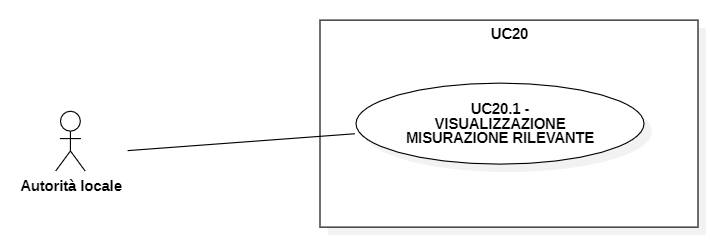
\includegraphics[width=0.9\textwidth]{../Images/subUC20.png}
    \caption{UC20.1 - VISUALIZZAZIONE MISURAZIONE RILEVANTE}
\end{figure}

%---------------------------- UC20.1 ---------------------------------

\subsubsection{UC20.1 - VISUALIZZAZIONE MISURAZIONE RILEVANTE}
\begin{itemize}
    \item \textbf{Attore principale:} Autorità locale;
    \item \textbf{Precondizioni:}
        \begin{itemize}
                \item L'autorità locale accede alla lista delle misurazioni rilevanti (UC20);
        \end{itemize}
    \item \textbf{Postcondizioni:}
        \begin{itemize}
                \item L'autorità locale visualizza una misurazione all'interno della lista delle misurazioni rilevanti.
        \end{itemize}
    \item \textbf{Scenario principale:}
        \begin{enumerate}
                \item Il sistema carica la lista delle misurazioni rilevanti.
        \end{enumerate}
\end{itemize}

%---------------------------- SUB_UC20.1 ---------------------------------

\begin{figure}[H]
    \centering
    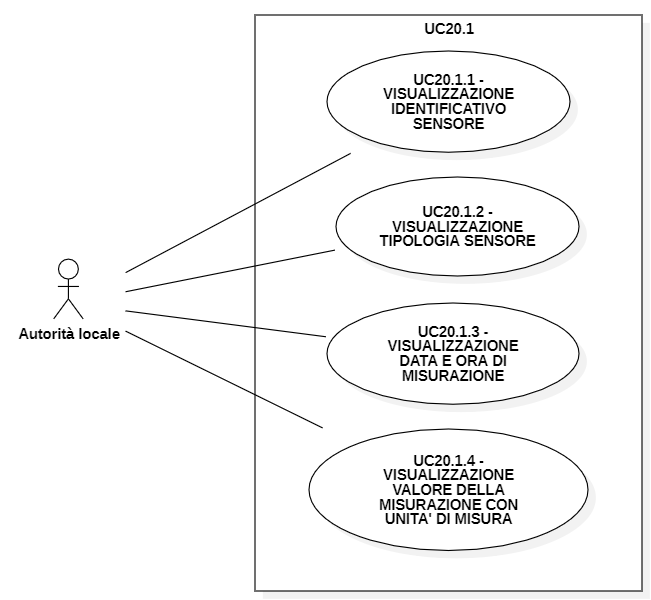
\includegraphics[width=0.9\textwidth]{../Images/subUC20.1.png}
    \caption{SOTTOCASI UC20.1 - VISUALIZZAZIONE MISURAZIONE RILEVANTE}
\end{figure}

%---------------------------- UC20.1.1 ---------------------------------

\subsubsection{UC20.1.1 - VISUALIZZAZIONE WIDGET LISTA RILEVANTI}
\begin{itemize}
      \item \textbf{Attore principale:} Autorità locale;
      \item \textbf{Precondizioni:}
            \begin{itemize}
                  \item Il sistema ha caricato la visualizzazione della dashboard (UC1);
            \end{itemize}
      \item \textbf{Postcondizioni:}
            \begin{itemize}
                  \item L'autorità locale visualizza la lista delle misurazioni rilevanti.
            \end{itemize}
      \item \textbf{Scenario principale:}
            \begin{enumerate}
                  \item L'autorità locale seleziona la visualizzione della lista delle misurazioni rilevanti.
            \end{enumerate}
      \item \textbf{User story associata:} \\
      Come autorità locale, desidero poter visualizzare una lista delle misurazioni rilevanti, al fine di reperire rapidamente delle misurazioni ritenute importanti.
\end{itemize}

%---------------------------- UC20.1.2 ---------------------------------

\subsubsection{UC20.1.2 - VISUALIZZAZIONE TIPOLOGIA SENSORE}
\begin{itemize}
    \item \textbf{Attore principale:} Autorità locale;
    \item \textbf{Precondizioni:}
        \begin{itemize}
                \item L'autorità locale visualizza una misurazione all'interno della lista delle misurazioni rilevanti (UC20.1);
        \end{itemize}
    \item \textbf{Postcondizioni:}
        \begin{itemize}
            \item L'autorità locale visualizza la tipologia del \textit{sensore}\textsubscript{\textit{G}} associato alla misurazione attualmente visualizzata all'interno della lista delle misurazioni rilevanti.
        \end{itemize}
    \item \textbf{Scenario principale:}
        \begin{enumerate}
            \item Il \textit{sistema}\textsubscript{\textit{G}} effettua il caricamento delle informazioni associate alla misurazione rilevante.
        \end{enumerate}
    \item \textbf{User story associata:} \\
    Come autorità locale, desidero poter visualizzare la tipologia del \textit{sensore}\textsubscript{\textit{G}} associato alla misurazione rilevante così da poter distinguere la tipologia della misurazione all'interno della lista delle misurazioni rilevanti, la quale contiene misurazioni provenienti da sensori di diversa tipologia.
\end{itemize}

%---------------------------- UC20.1.3 ---------------------------------

\subsubsection{UC20.1.3 - VISUALIZZAZIONE VALORE DELLA MISURAZIONE CON UNITÀ DI MISURA}
\begin{itemize}
    \item \textbf{Attore principale:} Autorità locale;
    \item \textbf{Precondizioni:}
        \begin{itemize}
                \item L'autorità locale visualizza una misurazione all'interno della lista delle misurazioni rilevanti (UC20.1);
        \end{itemize}
    \item \textbf{Postcondizioni:}
        \begin{itemize}
            \item L'autorità locale visualizza il valore con unità di misura della misurazione attualmente visualizzata all'interno della lista delle misurazioni rilevanti.
        \end{itemize}
    \item \textbf{Scenario principale:}
        \begin{enumerate}
            \item Il sistema effettua il caricamento delle informazioni associate alla misurazione rilevante.
        \end{enumerate}
    \item \textbf{User story associata:} \\
    Come autorità locale, desidero poter visualizzare il valore con unità di misura della misurazione rilevante.
\end{itemize}

%---------------------------- UC20.1.4 ---------------------------------

\subsubsection{UC20.1.4 - VISUALIZZAZIONE VALORE DELLA MISURAZIONE CON UNITÀ DI MISURA}
\begin{itemize}
    \item \textbf{Attore principale:} Autorità locale;
    \item \textbf{Precondizioni:}
        \begin{itemize}
                \item L'autorità locale visualizza una misurazione all'interno della lista delle misurazioni rilevanti (UC20.1);
        \end{itemize}
    \item \textbf{Postcondizioni:}
        \begin{itemize}
            \item L'autorità locale visualizza il valore con unità di misura della misurazione attualmente visualizzata all'interno della lista delle misurazioni rilevanti.
        \end{itemize}
    \item \textbf{Scenario principale:}
        \begin{enumerate}
            \item Il sistema effettua il caricamento delle informazioni associate alla misurazione rilevante.
        \end{enumerate}
    \item \textbf{User story associata:} \\
    Come autorità locale, desidero poter visualizzare il valore con unità di misura della misurazione rilevante.
\end{itemize}

%---------------------------- UC21 ---------------------------------
\newpage

\begin{figure}[H]
    \centering
    \includegraphics[width=0.9\textwidth]{../Images/uc21.PNG}
    \caption{UC21 - RIMOZIONE MISURAZIONE DA LISTA RILEVANTI}
\end{figure}
\subsubsection{UC21 - RIMOZIONE MISURAZIONE DA LISTA RILEVANTI}
\begin{itemize}
    \item \textbf{Attore principale:} Autorità locale;
    %\item \textbf{Descrizione:} L’autorità locale, dalla pagina adibita alla visione dei dati salvati tra i preferiti, rimuove un dato dalla lista.
    \item \textbf{Scenario principale:}
          \begin{enumerate}
            %  \item L'utente accede alla piattaforma per la visualizzazione della dashboard sullo stato della città o di una cella(UC1) (UC1.1);
             % \item L'utente sceglie di visualizzare la pagina dedicata alla visualizzazione dei dati preferiti;
              \item L'utente rimuove uno dei dati dalla lista.
          \end{enumerate}
    \item \textbf{Precondizioni:}
          \begin{itemize}
              \item  L'utente di trova nella pagina per la visulizzazione dei dati preferiti. (UC9)
              \item Almeno una misurazione è presente nella lista rilevanti.
          \end{itemize}
    \item \textbf{Postcondizioni:}
          \begin{itemize}
              \item  La misurazione viene rimosso dalla lista dei preferiti.
          \end{itemize}
    \item \textbf{User story associata:}
          \begin{itemize}
              \item Come autorità locale,
                    Desidero poter rimuovere un dato dalla lista dei preferiti sulla piattaforma,
                    Per poter gestire in modo efficiente i dati visualizzati sulla dashboard.
          \end{itemize}
\end{itemize}

%---------------------------- UC22 ---------------------------------

\begin{figure}[H]
    \centering
    \includegraphics[width=0.9\textwidth]{../Images/uc22.PNG}
    \caption{UC22 - VISUALIZZAZIONE ALLERTE SUPERAMENTO SOGLIE}
\end{figure}
\subsubsection{UC22 - VISUALIZZAZIONE ALLERTE SUPERAMENTO SOGLIE}
\begin{itemize}
      \item \textbf{Attore principale:} Autorità locale;
      \item \textbf{Precondizioni:}
            \begin{itemize}
                  \item Il sensore ha registrato una misurazione al di sopra o al di sotto di una soglia specifica.
            \end{itemize}
      \item \textbf{Postcondizioni:}
            \begin{itemize}
                  \item  L'autorità locale riceve una notifica di superamento di una soglia impostata.
            \end{itemize}
      \item \textbf{Scenario principale:}
            \begin{enumerate}
                  \item  Il sistema rileva condizioni che richiedono l'invio di una notifica per segnalare il superamento di una soglia impostata;
                  \item Il sistema inivia una notifica all'autorità locale.
            \end{enumerate}
      \item \textbf{User story associata:}
      Come autorità locale, desidero ricevere notifiche immediate nel caso in cui le misurazioni superino le soglie di sicurezza superiori o scendano al di sotto delle soglie di sicurezza inferiori, permettendomi di adottare prontamente azioni correttive e necessarie.
\end{itemize}

%---------------------------- UC23 ---------------------------------

\begin{figure}[H]
    \centering
    \includegraphics[width=0.9\textwidth]{../Images/uc23.PNG}
    \caption{UC23 - TRASMISSIONE DATI TEMPERATURA}
\end{figure}
\subsubsection{UC23 - TRASMISSIONE DATI TEMPERATURA}
\begin{itemize}
    \item \textbf{Attore principale:} Sensore;
    \item \textbf{Precondizioni:}
        \begin{itemize}
            \item Il \textit{sensore}\textsubscript{\textit{G}} è attivo e connesso al \textit{sistema}\textsubscript{\textit{G}}. 
        \end{itemize}
    \item \textbf{Postcondizioni:}
        \begin{itemize}
            \item Il \textit{sistema}\textsubscript{\textit{G}} ha memorizzato ed elaborato i dati inviati dal \textit{sensore}\textsubscript{\textit{G}}.
        \end{itemize}
    \item \textbf{Scenario principale:}
        \begin{enumerate}
            \item Il \textit{sensore}\textsubscript{\textit{G}} effettua un rilevamento della temperatura;
            \item Il \textit{sensore}\textsubscript{\textit{G}} formatta il messaggio da trasmettere al \textit{sistema}\textsubscript{\textit{G}} contenente l'identificativo del \textit{sensore}\textsubscript{\textit{G}} e la misurazione effettuata in gradi Celsius;
            \item Il \textit{sensore}\textsubscript{\textit{G}} trasmette il messaggio al \textit{sistema}\textsubscript{\textit{G}}.
        \end{enumerate}
    \item \textbf{User story associata:} \\
    Come Sensore, desidero trasmettere i rilevamenti di temperatura al \textit{sistema}\textsubscript{\textit{G}}.
\end{itemize}


%---------------------------- UC24 ---------------------------------

\begin{figure}[H]
    \centering
    \includegraphics[width=0.9\textwidth]{../Images/uc24.PNG}
    \caption{UC24 - TRASMISSIONE DATI UMIDITA'}
\end{figure}
\subsubsection{UC24 - TRASMISSIONE DATI UMIDITA'}
\begin{itemize}
    \item \textbf{Attore principale:} Sensore;
    \item \textbf{Precondizioni:}
        \begin{itemize}
            \item Il sensore è attivo e connesso al sistema. 
        \end{itemize}
    \item \textbf{Postcondizioni:}
        \begin{itemize}
            \item Il sistema ha memorizzato ed elaborato i dati inviati dal sensore.
        \end{itemize}
    \item \textbf{Scenario principale:}
        \begin{enumerate}
            \item Il sensore effettua un rilevamento dell'umidità nell'aria;
            \item Il sensore formatta il messaggio da trasmettere al sistema contenente l'identificativo del sensore e la misurazione effettuata in percentuale di umidità nell’aria;
            \item Il sensore trasmette il messaggio al sistema.
        \end{enumerate}
    \item \textbf{User story associata:} \\
    Come Sensore, desidero trasmettere i rilevamenti dell'umidità nell'aria al sistema.
\end{itemize}


%---------------------------- UC25 ---------------------------------

\begin{figure}[H]
    \centering
    \includegraphics[width=0.9\textwidth]{../Images/uc25.PNG}
    \caption{UC25 - TRASMISSIONE LIVELLO ACQUA}
\end{figure}
\subsubsection{UC25 - TRASMISSIONE DATI LIVELLO ACQUA}
\begin{itemize}
    \item \textbf{Attore principale:}Sensore;
    %\item \textbf{Descrizione:} L’autorità locale, dalla pagina adibita alla visione dei dati salvati tra i preferiti, rimuove un dato dalla lista.
    \item \textbf{Scenario principale:}
          \begin{enumerate}
              \item Il sensore effettua una rilevazione del livello dell'acqua;
              \item Il sensore formatta il messaggio da inviare al sistema;
              \item Il sensore invia il messaggio al sistema
          \end{enumerate}
    \item \textbf{Precondizioni:}
          \begin{itemize}
              \item  il sensore è attivito e connesso al sistema. 
          \end{itemize}
    \item \textbf{Postcondizioni:}
          \begin{itemize}
              \item  il sistema ha memorizzato ed elaborato i dati inviati dal sensore.
          \end{itemize}
    \item \textbf{User story associata:}
          \begin{itemize}
            \item  Come Sensore, voglio trasmettere in modo affidabile i dati di del livello dell'acqua al sistema, in modo che possano essere memorizzati e elaborati 
          \end{itemize}
\end{itemize}


%---------------------------- UC26 ---------------------------------

\begin{figure}[H]
    \centering
    \includegraphics[width=0.9\textwidth]{../Images/uc26.PNG}
    \caption{UC26 - TRASMISSIONE DATI ISOLE ECOLOGICHE}
\end{figure}
\subsubsection{UC26 - TRASMISSIONE DATI ISOLE ECOLOGICHE}
\begin{itemize}
    \item \textbf{Attore principale:}Sensore;
    %\item \textbf{Descrizione:} L’autorità locale, dalla pagina adibita alla visione dei dati salvati tra i preferiti, rimuove un dato dalla lista.
    \item \textbf{Scenario principale:}
          \begin{enumerate}
              \item Il sensore effettua una rilevazione sullo stato di riempimento delle isole ecologiche;
              \item Il sensore formatta il messaggio da inviare al sistema;
              \item Il sensore invia il messaggio al sistema
          \end{enumerate}
    \item \textbf{Precondizioni:}
          \begin{itemize}
              \item  il sensore è attivito e connesso al sistema. 
          \end{itemize}
    \item \textbf{Postcondizioni:}
          \begin{itemize}
              \item  il sistema ha memorizzato ed elaborato i dati inviati dal sensore.
          \end{itemize}
    \item \textbf{User story associata:}
          \begin{itemize}
            \item Come Sensore, voglio trasmettere in modo affidabile i dati di riempimento delle isole ecologiche al sistema, in modo che possano essere memorizzati e elaborati 
          \end{itemize}
\end{itemize}


%---------------------------- UC27 ---------------------------------

\begin{figure}[H]
    \centering
    \includegraphics[width=0.9\textwidth]{../Images/uc27.PNG}
    \caption{UC27 - TRASMISSIONE DATI COLONNINE DI RICARICA}
\end{figure}
\subsubsection{UC27 - TRASMISSIONE DATI COLONNINE DI RICARICA}
\begin{itemize}
    \item \textbf{Attore principale:} Sensore;
    \item \textbf{Precondizioni:}
        \begin{itemize}
            \item Il sensore è attivo e connesso al sistema. 
        \end{itemize}
    \item \textbf{Postcondizioni:}
        \begin{itemize}
            \item Il sistema ha memorizzato ed elaborato i dati inviati dal sensore.
        \end{itemize}
    \item \textbf{Scenario principale:}
        \begin{enumerate}
            \item Il sensore effettua un rilevamento sull'occupazione delle colonnine di ricarica;
            \item Il sensore formatta il messaggio da trasmettere al sistema;
            \item Il sensore trasmette il messaggio al sistema.
        \end{enumerate}
    \item \textbf{User story associata:} \\
    Come Sensore, desidero trasmettere con affidabilità i rilevamenti sull'occupazione delle colonnine di ricarica, garantendo che siano memorizzati e processati correttamente.
\end{itemize}

%---------------------------- UC28 ---------------------------------

\begin{figure}[H]
    \centering
    \includegraphics[width=0.9\textwidth]{../Images/uc28.PNG}
    \caption{UC28 - TRASMISSIONE DATI POLVERI SOTTILI}
\end{figure}
\subsubsection{UC28 - TRASMISSIONE DATI POLVERI SOTTILI}
\begin{itemize}
    \item \textbf{Attore principale:} Sensore;
    \item \textbf{Precondizioni:}
        \begin{itemize}
            \item Il sensore è attivo e connesso al sistema. 
        \end{itemize}
    \item \textbf{Postcondizioni:}
        \begin{itemize}
            \item Il sistema ha memorizzato ed elaborato i dati inviati dal sensore.
        \end{itemize}
    \item \textbf{Scenario principale:}
        \begin{enumerate}
            \item Il sensore effettua un rilevamento della quantità di particelle di polveri nell'aria;
            \item Il sensore formatta il messaggio da trasmettere al sistema;
            \item Il sensore trasmette il messaggio al sistema.
        \end{enumerate}
    \item \textbf{User story associata:} \\
    Come Sensore, desidero trasmettere i rilevamenti della quantità di particelle di polveri nell'aria al sistema.
\end{itemize}


%---------------------------- UC29 ---------------------------------

\begin{figure}[H]
    \centering
    \includegraphics[width=0.9\textwidth]{../Images/uc29.PNG}
    \caption{UC29 - TRASMISSIONE DATI GUASTI ELETTRICI}
\end{figure}
\subsubsection{UC29 - TRASMISSIONE DATI GUASTI ELETTRICI}
\begin{itemize}
    \item \textbf{Attore principale:} Sensore;
    \item \textbf{Precondizioni:}
        \begin{itemize}
            \item Il sensore è attivo e connesso al sistema. 
        \end{itemize}
    \item \textbf{Postcondizioni:}
        \begin{itemize}
            \item Il sistema ha memorizzato ed elaborato i dati inviati dal sensore.
        \end{itemize}
    \item \textbf{Scenario principale:}
        \begin{enumerate}
            \item Il sensore effettua un rilevamento della presenza di guasti elettrici;
            \item Il sensore formatta il messaggio da trasmettere al sistema;
            \item Il sensore trasmette il messaggio al sistema.
        \end{enumerate}
    \item \textbf{User story associata:} \\
    Come Sensore, desidero trasmettere i rilevamenti della presenza di guasti elettrici.
\end{itemize}


\newcounter{rowcounter}
\setcounter{rowcounter}{1}



\newpage
\section{Requisiti}
Per poter utilizzare il software occorre rispettare i seguenti
requisiti minimi:  

\subsection{Requisiti hardware}
L’applicazione esegue su \textit{browser}\textsubscript{\textit{G}}, come tale non si individuano dei requisiti specifici, fissati da parte
della \textit{proponente}\textsubscript{\textit{G}}, dal capitolato o dal progetto stesso. I seguenti, pertanto, sono individuati come
riferimento di massima per l’esecuzione del prodotto creato.   
\begin{table}[H]
    \centering
    \begin{tabular}{ll}
        \toprule
        \textbf{Componente} & \textbf{Requisito} \\
        \midrule
        Processore & \textit{Dual-core CPU}\textsubscript{\textit{G}}, \textit{clock rate}\textsubscript{\textit{G}}: 1.5 GHz \\
        Memoria & 2 GB di RAM \\
        Spazio su disco & 10 GB di spazio disponibile\\
        \bottomrule
    \end{tabular}
    \caption{Requisiti hardware minimi}
\end{table} 
\subsubsection{Requisiti software}
Di seguito sono elencati i \textit{browser}\textsubscript{\textit{G}} per i quali è garantita la compatibilità con il dispositivo (desktop o mobile). È importante notare che l'applicazione potrebbe funzionare anche su altri \textit{browser}\textsubscript{\textit{G}} o versioni precedenti, ma non è garantito il pieno supporto.  
\begin{table}[H]
    \centering
    \begin{tabular}{ll}
        \toprule
        \textbf{Browser} & \textbf{Versione} \\
        \midrule
        \textit{Chrome}\textsubscript{\textit{G}} & v.89.0.4389.82\\
        \textit{Firefox}\textsubscript{\textit{G}} & v.86.0 \\
        \textit{Safari}\textsubscript{\textit{G}} & v.14.0 \\
        \textit{Edge}\textsubscript{\textit{G}} & v.89.0.774.54 \\
        \bottomrule
    \end{tabular}
    \caption{Browser e versioni supportate}
\end{table}

Inoltre, vengono indicate le versioni minime dei sistemi operativi necessarie per poter utilizzare l'applicazione. Come avviene per i \textit{browser}\textsubscript{\textit{G}}, l'applicazione potrebbe operare su sistemi operativi differenti o su versioni precedenti, tuttavia, non è garantito il completo supporto.\\
\begin{table}[H]
    \centering
    \begin{tabular}{ll}
        \toprule
        \textbf{OS} & \textbf{Versione} \\
        \midrule
        \textit{Linux}\textsubscript{\textit{G}} & Ubuntu: versione 18.04 LTS\\&Debian: versione 9\\& RHEL: versione 7\\& CentOS: versione 7\\& Fedora: versione 30 \\
        \textit{Windows}\textsubscript{\textit{G}} & \textit{Windows}\textsubscript{\textit{G}} 10, \textit{Windows}\textsubscript{\textit{G}} Server 2012 R2 \\
        \textit{MacOS}\textsubscript{\textit{G}} & macOS 10.13 (High Sierra) \\
        \bottomrule
    \end{tabular}
    \caption{Sistemi operativi e versioni supportate}
\end{table} 



\end{document}